%&../.preamble

\externalize{../.preamble}

\usepackage{pifont}
\usepackage{makecell}
\usepackage{contour}
% \usepackage{amssymb}        % gives \bigstar
\definecolor{score1}{rgb}{0.70, 0.30, 0.30} % muted red
\definecolor{score2}{rgb}{0.75, 0.40, 0.30}
\definecolor{score3}{rgb}{0.80, 0.50, 0.30}
\definecolor{score4}{rgb}{0.85, 0.60, 0.30}
\definecolor{score5}{rgb}{0.90, 0.70, 0.30} % warm muted orange
\definecolor{score6}{rgb}{0.90, 0.75, 0.30}
\definecolor{score7}{rgb}{0.85, 0.80, 0.35}
\definecolor{score8}{rgb}{0.75, 0.80, 0.40}
\definecolor{score9}{rgb}{0.60, 0.75, 0.40}
\definecolor{score10}{rgb}{0.45, 0.70, 0.40} % muted green

\title{Pelstra di algoritmi}
\author{Marini Mattia}
\date{20 ottobre 2025}

\begin{document}
\maketitle
\license{Palestra di algoritmi}
\tableofcontents
\newpage

\section{Introduzione}
Qui di seguito sono raccolte nozioni di base per affrontare ogni probrema relativo alle \textit{OII}

\subsection{Basi cpp}
In ogni problema è necessario effettuare input/output su file\footnote{In realtà a volte è sufficiente implementare il body di una funzione oppure la parte relativa all'output viene fornita}. Ci sono diversi modi per eseguire ciò.
\subsubsection{Input metodo 1 (consigliato)}
Vedi file \href{run:./files/teoria/input1/}{input1.cpp}
\vskip3mm
L'idea è di creare un oggeto \verb|ifstream| e \verb|ofstream| che poi potremmo utilizzare in maniera totalmente analoga a, rispettivamente, \verb|cin| e \verb|cout|
\begin{lstlisting}[language = cpp, frame = none]
std::ifstream in("input.txt");
in >> a >> b;

std::ifstream out("output.txt");
out << a << b
\end{lstlisting}
Esiste un trucco per velocizzare notevolmente la velocità di input/output utilizzando questo metodo. In particolare, è sufficiente appendere le seguenti righe prima di scrivere o leggere su files:
\begin{lstlisting}[language = cpp, frame = none]
ios_base::sync_with_stdio(false); 
cin.tie(NULL);
\end{lstlisting}
Tuttavia se il problema sfora i limiti di tempo, con ogni probabilità è la soluzione a non essere corretta, non le operazioni di input/output. Queste righe possono essere utili per scalare la classifica sui siti di allenamento, non per altro

\subsubsection{Input metodo 2}
Vedi file \href{run:./files/teoria/input/}{input2.cpp}
\vskip3mm
Questo metodo è più "vecchio" e meno consigliato. L'idea è di utilizzare le funzioni \verb|freopen| per reindirizzare lo standard input/output su file:
\begin{lstlisting}[language = cpp, frame = none]
FILE *in = fopen("input.txt", "r");
fscanf(in, "%d %d", &a, &b);

FILE *out = fopen("output.txt", "w");
fprintf(out, "%d %d\n", a, b);
\end{lstlisting}
dove le funzioni \verb|fprintf| e \verb|fscanf| prendono come argomenti:
\begin{itemize}
	\item Il puntatore ad un file \verb|FILE *|
	\item Una stringa \verb|format|, contenente una serie di specificatori, preceduti da "{\ttfamily \%}"
	      \begin{itemize}
		      \item \verb|d|: decimal, numero intero
		      \item \verb|f|: float
		      \item \verb|s|: stringa c-style, in particolare \verb|char *|
	      \end{itemize}
	\item Una serie variabili che corrispondono a quanto indicato in \verb|format|. Nel caso di \verb|scanf| è richiesto l'indirizzo di memoria di queset
\end{itemize}
\subsubsection{Ultra fast io}
Ci sono infine alcuni metodi per velocizzare l'input al massimo, utili per sprepere la perfomance al massimo, per arrivare nei primi in classifica. In particolare, questi metodi si basano sull'uso delle funzioni \verb|getchat_unlocked()| e \verb|putchar_unlocked()|
\begin{lstlisting}[language = cpp, frame = none]
inline static int scanInt(FILE *file = stdin) {
  int n = 0;
  int neg = 1;
  char c = getc_unlocked(file);
  if (c == '-')
    neg = -1;
  while (c < '0' || c > '9') {
    c = getc_unlocked(file);
    if (c == '-')
      neg = -1;
  }
  while (c >= '0' && c <= '9') {
    n = (n << 3) + (n << 1) + c - '0';
    c = getc_unlocked(file);
  }
  return n * neg;
}

inline static void writeInt(int v, FILE *file = stdout) {
  static char buf[14];
  int p = 0;
  if (v == 0) {
    putc_unlocked('0', file);
    return;
  }
  if (v < 0) {
    putc_unlocked('-', file);
    v = -v;
  }
  while (v) {
    buf[p++] = v % 10;
    v /= 10;
  }
  while (p--) {
    putc_unlocked(buf[p] + '0', file);
  }
}

inline static int getString(char *buf, FILE *file = stdin) {
  std::string s;
  int c = getc_unlocked(file);

  // Skip leading whitespace
  while (c != EOF && (c == ' ' || c == '\n' || c == '\t' || c == '\r'))
    c = getc_unlocked(file);

  // Read until next whitespace or EOF
  int index = 0;
  while (c != EOF && c != ' ' && c != '\n' && c != '\t' && c != '\r') {
    buf[index++] = static_cast<char>(c);
    c = getc_unlocked(file);
  }

  return index;
}

inline static void putString(const std::string &s, FILE *file = stdout) {
  for (size_t i = 0; i < s.size(); i++)
    putc_unlocked(s[i], file);
}
\end{lstlisting}
Nota che le funzioni \verb|putc_unlocked| e \verb|getc_unlocked| sono disponibili solo in sistemi operativi unix(MacOs e Linux). Si possono usare in tranquillità dato che i server che testano il nostro codice sono tutti linux, ma il codice potrebbe non compilare in locale

\subsection{Complessità}
Il punto focale delle olimpiadi di informatica è non solo quello di scrivere algoritmi funzionanti, bensì efficienti. Per questa ragione è importante fornire critesi secondo i quali valutare la velocità d'esecuzione degli algoritmi
\vskip3mm
La logica di base sta nel relazionare il \textit{numero di iterazioni} che un algoritmo deve eseguire alla \textit{dimensione dell'input}.

\subsubsection{Esempio 1}
Supponiamo di avere un algoritmo per trovare il massimo in un vettore di $ n $ elementi. L'algoritmo fa quanto segue:
\begin{itemize}
	\item Inizializza una variabile \verb|max| al primo elemento del vettore
	\item Per ogni elemento del vettore controlla se è maggiore di \verb|max|. In caso affermativo aggiorna \verb|max| all'elemento corrente
	\item Ritorna \verb|max|
\end{itemize}
\begin{algoritmo*}{Massimo vettore}
	\begin{algorithm}[H]
		\SetKwFunction{Max}{\Int max}
		\Fn{ \Max{$\Int\ v[]$}}{
			$max \gets v\left[0\right]$\;
			\For{$i = 0$ \KwTo $v.size - 1$}{
				\If{$v\left[i\right] > max$}{
					$max \gets v\left[i\right]$\;
				}
			}
			\Return{$max$}\;
		}
	\end{algorithm}
\end{algoritmo*}
In questo caso notiamo come siano necessarie $ n $ \textit{iterazioni} perchè l'algoritmo termini (dove $ n $ è la dimensione del vettore $ v $). Abbiamo quindi rapportato la dimensione dell'input alla complessità temporale dell'algoritmo
\vskip3mm
In questo caso, si dice che la complessità dell'algoritmo è $ \Theta \left(n\right) $

\subsubsection{Esempio 2}
Supponiamo di avere un algorimo che debba eseguire una moltiplicazione applicando la proprietà distributiva:
\[
	\left(a + b + c\right)\cdot \left(d + e + f\right)
\]
secondo la proprietà distributiva questo diventa:
\[
	\underbracket[0.1ex]{\left(ad + ae + af\right)}_{A}+ \underbracket[0.1ex]{\left(bd + be + bf\right)}_{B} + \underbracket[0.1ex]{\left(cd + ce + cf\right)}_{C}
\]
ritornare un vettore che contenga i coefficienti $ \left(A,B,C\right) $

\begin{algoritmo*}{Moltiplicazione distributiva}
	\begin{algorithm}[H]
		\SetKwFunction{Mul}{\Int mul}
		\Fn{ \Mul{$\Int\ v_1[]$, $\Int\ v_2[]$}}{
		$\Int\; rv$ = $\Int[0 \ldots v1.size]$\;
		\For{$i = 0$ \KwTo $v_1.size - 1$}{
			$ rv\left[i\right] = 0$\;
			\For{$j = 0$ \KwTo $v_2.size - 1$}{
				$ rv += v_1\left[i\right] \cdot  v_2\left[j\right] $\;
			}
		}
		\Return{$rv$}\;
		}
	\end{algorithm}
\end{algoritmo*}
Siccome per ogni elemento di $ v_1 $ devo scorrere interamente $ v_2 $, dovro ripetere $ v_2 * v_1 $ volte il body del ciclo.
\vskip3mm
In questo caso, se i due vettori hanno dimensione $ n $, si dice che la complessità dell'algoritmo è $ \Theta \left(n^2 \right) $

\subsubsection*{Notazione $ \Omega $, $ \Theta $, $ O $}
In generale, per valutare la complessità di un algoritmo siamo interessati a più scenari:
\begin{itemize}
	\item Nel peggiore dei casi, l'algoritmo che complessità ha? $ \rightarrow  $ notazione $ O $
	\item Nel migliore dei casi, l'algoritmo che complessità ha?$ \rightarrow  $ notazione $ \Omega  $
	\item Nel "caso medio", l'algoritmo che complessità ha?$ \rightarrow  $ notazione $ \Theta $
\end{itemize}
Nota bene: nella maggio parte dei casi siamo interessati alla coplessità nel caso pessimo $ O $ in quanto non possiamo escludere che questo si presenti nel dataset.
\vskip3mm
Per capire meglio la differenza fra caso ottimo e caso pessimo prendiamo in analisi l'algoritmo di \textit{insertion sort}:

\begin{algoritmo*}{Insertion Sort}
	\begin{algorithm}[H]
		\SetKwFunction{InsertSort}{insertionSort}
		\Fn{\Int \InsertSort{$\Int\ v[]$}}{
			\For{$i = 1$ \KwTo $v.size - 1$}{
				$\Int\ key = v[i]$\;
				$\Int\ j = i - 1$\;
				\While{$j \geq 0$  \And  $v[j] > key$}{
					$v[j + 1] = v[j]$\;
					$j = j - 1$\;
				}
				$v[j + 1] = key$\;
			}
			\Return{$v$}\;
		}
	\end{algorithm}
\end{algoritmo*}
In questo caso, dato un vettore lungo $ n $, abbiamo due casi estremi:
\begin{itemize}
	\item Il vettore è ordinato in modo crescente
	\item Il vettore è ordinato in modo decrescente
\end{itemize}
Nel primo caso l'algoritmo non entrerà mai nel ciclo while e dunque scorrerà il vettore una singola volta, originando una compessità di $ \Omega \left(n\right) $.
\vskip3mm
Nel secondo caso l'algoritmo dovrà per ogni elemento del vettore scorrere (quasi) tutto il vettore stesso, originando una complessità di $ O\left(n^2 \right) $

\subsection{Struttura problemi}
Ogni problema delle OII e delle OIS ha una struttura simile e si compone come segue:
\begin{itemize}
	\item Descrizione problema
	\item Descrizione dati di input
	\item Descrizione formato output
	\item Esempi
	\item Testcase
\end{itemize}
In particolare, il punteggio viene assegnato in base ai testcase che il nostro codice passa. Dobbiamo quindi scrivere un codice che risolva un dato problema stampando in output la soluzione. La correzione funziona come segue:
\begin{itemize}
	\item I testcase sono raggruppati in un dato numero di \textit{gruppi}
	\item Ad ogni gruppo di \textit{testcase} è assegnato un punteggio e delle assunzioni. Ad esempio, ci può essere detto che i dati in input, in un dato gruppo non superano una certa dimensione o sono strutturati in un modo particolare
	\item Se all'interno di un gruppo i testcase sono tutti passati (output corretto), allora vengono assegnati i punti, altrimenti no
\end{itemize}
Si noti che per passare un testcase non è sufficiente che l'output sia corretto, ma il tempo di esecuzione e la memoria utilizzata devono essere entro i limiti previsti, specificati nel testo del problema

\section{Programmazione dinamica}

\subsection{Donimo}
Quanti modi ho di disporre tasselle di domino in una scacchiera $ 2 \times n $?

\vskip3mm\sfblue{Soluzione}\vskip3mm
\begin{itemize}
	\item Salvo in $ dp\left[i\right] $ il numero di combinazioni che ci sono per un rettangolo $ 2 \times i $
	\item Ho due opzioni:
	      \begin{itemize}
		      \item Metto 2 tessere in orizzontale, allora $ dp\left[i\right] = dp\left[i-2\right] $
		      \item Metto 1 tessera in verticale, allora $ dp\left[i\right] = dp\left[i-1\right] $
	      \end{itemize}
	\item Quindi $ dp\left[i\right] = dp\left[i-1\right] + dp\left[i-2\right] $
	\item La soluzione è $ \operatorname{Fib}\left(n\right) $
\end{itemize}
\subsection{Hateville}
Ho un vettore di prezzi. Se prendo un prezzo $ v\left[i\right] $ non posso prendere $ v\left[i-1\right] $ e $ v\left[i+1\right] $. Trova prezzo massimo

\vskip3mm\sfblue{Soluzione}\vskip3mm
\begin{itemize}
	\item Salvo in $ dp\left[i\right] $ il prezzo massimo che posso ottenere con i vicini $ \le i $
	\item Ho due opzioni:
	      \begin{itemize}
		      \item Non prendo $ v\left[i\right] $, allora il prezzo è $ dp\left[i-1\right] $
		      \item Prendo $ v\left[i\right] $, allora il prezzo è $ dp\left[i-1\right] + v\left[i\right] $
	      \end{itemize}
\end{itemize}
\subsection{Zaino}\label{zaino}
Zaino ha capacità $ C $, ho $ n $ pezzi di peso $ w\left[i\right] $ e profitto $ p\left[i\right] $. Trova profitto massimo

\vskip3mm\sfblue{Soluzione}\vskip3mm
\begin{itemize}
	\item Crea matrice $ n \times C $ in cui si salva $ dp\left[i\right]\left[j\right] $ il profitto massimo che si può ottenere con i pezzi $ \le i $ e capacità $ \le j $
	\item Ho due opzioni:
	      \begin{itemize}
		      \item Prendo pezzo $ \left(i,j\right) $, allora il prezzo migliore è $ dp\left[i-1\right]\left[j - w\left[i\right]\right] + p\left[i\right] $
		      \item Non lo prendo, allora il prezzo è $ dp\left[i-1\right]\left[j\right] $
	      \end{itemize}
	\item Posso ottimizzare lo spazio tenendo salvato solo due righe della matrice, la $ i $ e la $ i-1 $
\end{itemize}
\subsection{Zaino umbound}
Vedi \hyperref[zaino]{zaino}, solo che non c'è limite al numero di oggetti che uno puo prendere

\vskip3mm\sfblue{Soluzione}\vskip3mm
\begin{itemize}
	\item Vettore $ dp $ in cui salvo in $ i $ il profitto massimo per uno zaino grande $ i $
	\item Per ogni peso item $ x $, il profitto massimo è $ p\left[x\right] + dp\left[i - w\left[x\right]\right] $
	\item $ dp\left[i\right] $ è il massimo fra tutti i valori trovati al punto 2
\end{itemize}
\subsection{LCS}
Date due stringhe $ U $ e $ T $, trova la \underline{sottosequenza} massimale. Una sottosequenza è una stringa che si ottiene da un'altra selezionandone solo alcuni caratteri (non necessariamente contigui, ma mantenendone l'ordine).
\vskip3mm\sfblue{Soluzione}\vskip3mm
\begin{itemize}
	\item Tabella $ dp $ con $ U $ su un lato e $ T $ sull'altro. In $ dp\left[i\right]\left[j\right] $ salvo la lunghezza della $ LCS $ fra la sottostringa $ U\left[0,i\right] $ e $ T\left[0, j\right] $
	\item Ho due opzioni:
	      \begin{itemize}
		      \item $ U\left[i\right] = T[j] $, allora $ dp\left[i\right]\left[j\right] = dp\left[i-1\right]\left[j-1\right] +1 $ (aggiungo un carattere alla LCS più corta di 1)
		      \item $  U\left[i\right] \neq T[j] $  allora $ dp\left[i\right]\left[j\right] = \operatorname{max}\left(dp\left[i-1\right]\left[j\right], dp\left[i\right]\left[j-1\right]\right) $. Vedi immagine
	      \end{itemize}
\end{itemize}

\begin{center}
	\begin{tikzpicture}[scale=0.7]
		\draw [fill=mutedgreen!50](6, 0)rectangle ++ (2,1);
		\draw (0,0)grid(8,1);

		\draw [fill=mutedred!50](6, -3)rectangle ++ (4,1);
		\draw (0,-3)grid(10,-2);

		\begin{scope}[shift={(0.5,0.5)}]
			\node at (-1, 0) {$ U $};

			\node (1) at (0,0)  {a};
			\node (2) at (1,0)  {u};
			\node (3) at (2,0)  {t};
			\node (4) at (3,0)  {s};
			\node (5) at (4,0)  {s};
			\node (6) at (5,0)  {g};
			\node (7) at (6,0)  {n};
			\node (18) at (7,0)  {k};
			\node [anchor = south] at (7,0.5)  {$ i $};

			\node at (-1, -3) {$ V $};

			\node (8)  at (0,-3)  {w};
			\node (9)  at (1,-3)  {a};
			\node (10) at (2,-3)  {t};
			\node (11) at (3,-3)  {f};
			\node (12) at (4,-3)  {x};
			\node (13) at (5,-3)  {m};
			\node (14) at (6,-3)  {g};
			\node (15) at (7,-3)  {o};
			\node (16) at (8,-3)  {i};
			\node (17) at (9,-3)  {m};
			\node [anchor = south] at (6,-2.5)  {$ j $};
			% \node (15) at (7,-3)  {o};
			% \node (16) at (8,-3)  {i};

		\end{scope}

		\node (lcs)[circle] at (2,-1) {lcs};

		\draw (lcs)edge(1.south) edge (3.south) edge(6.south);
		\draw (lcs)edge(9.north) edge (10.north) edge(14.north);

	\end{tikzpicture}
\end{center}

Per migliorare la soluzione, se i caratteri sono diversi, devo aggiungere un carattere che sia nell'insieme dei caratteri dopo l'ultimo carattere comune. Quindi ho che
\begin{itemize}
	\item A $ T $, devo aggiungere un carattere che appartiene all'insieme rosso
	\item A $ U $, devo aggiungere un carattere che appartiene all'insieme verde
\end{itemize}
Chiaramente la cosa è asimmetrica, per questo devo controllare $ dp\left[i-1\right]\left[j\right] $ e $ dp\left[i\right]\left[j-1\right] $
\vskip3mm
\sfblue{Dimostrazione formale}: dobbiamo dimostrare che date due parole $ U \left(u_1,\ldots ,u_i\right) $ e $ V\left(v_1 , \ldots v_j\right) $ e $ X \left(x_1 , \ldots x_k\right) $ allora
\begin{itemize}
	\item Se $ u_i = v_j $  allora
	      \begin{gather*}
		      u_i = v_j = x_k \\
		      X\left(K-1\right) \in \mathcal{LCS}\left(U\left(i-1\right), V\left(j-1\right)\right)
	      \end{gather*}
	\item Se $ u_i \neq v_j $ e $ x_k \neq  u_i $ allora
	      \[
		      X \in \mathcal{LCS}\left(U\left(i-1\right), V \right)
	      \]
	\item Se $ u_i \neq v_j $ e $ x_k \neq  v_j $ allora
	      \[
		      X \in \mathcal{LCS}\left(U, V\left(j-1\right) \right)
	      \]
\end{itemize}

\begin{minipage}[t]{0.48\textwidth}
	\begin{center}
		\begin{tikzpicture}[scale=0.7]
			\draw (0,0)grid(8,1);
			\draw [fill=mutedgreen!50](7, 0)rectangle ++ (1,1);

			\draw (0,-3)grid(7,-2);
			\draw [fill=mutedred!50](6, -3)rectangle ++ (1,1);

			\begin{scope}[shift={(0.5,0.5)}]
				\node at (-1, 0) {$ U $};

				\node (1) at (0,0)  {a};
				\node (2) at (1,0)  {u};
				\node (3) at (2,0)  {t};
				\node (4) at (3,0)  {s};
				\node (5) at (4,0)  {s};
				\node (6) at (5,0)  {g};
				\node (7) at (6,0)  {n};
				\node (17) at (7,0)  {k};
				\node [anchor = south] at (7,0.5)  {$ i $};

				\node at (-1, -3) {$ V $};

				\node (8)  at (0,-3)  {w};
				\node (9)  at (1,-3)  {a};
				\node (10) at (2,-3)  {t};
				\node (11) at (3,-3)  {f};
				\node (12) at (4,-3)  {x};
				\node (13) at (5,-3)  {m};
				\node (14) at (6,-3)  {g};
				\node [anchor = south] at (6,-2.5)  {$ j $};
				% \node (15) at (7,-3)  {o};
				% \node (16) at (8,-3)  {i};

			\end{scope}

			\node (lcs)[circle] at (2,-1) {lcs};

			\draw (lcs)edge(1.south) edge (3.south) edge(6.south);
			\draw (lcs)edge(9.north) edge (10.north) edge(14.north);

		\end{tikzpicture}
	\end{center}
\end{minipage}
%
\begin{minipage}[t]{0.48\textwidth}
	\begin{center}
		\begin{tikzpicture}[scale=0.7]

			\draw (0,0)grid(6,1);
			\draw [fill=mutedblue!50](5, 0)rectangle(6,1);

			\draw (0,-3)grid(7,-2);
			\draw [fill=mutedblue!50](6, -3)rectangle(7,-2);

			\begin{scope}[shift={(0.5,0.5)}]
				\node at (-1, 0) {$ U $};

				\node (1) at (0,0)  {a};
				\node (2) at (1,0)  {u};
				\node (3) at (2,0)  {t};
				\node (4) at (3,0)  {s};
				\node (5) at (4,0)  {s};
				\node (6) at (5,0)  {g};
				\node [anchor = south] at (5,0.5)  {$ i $};

				\node at (-1, -3) {$ V $};

				\node (8)  at (0,-3)  {w};
				\node (9)  at (1,-3)  {a};
				\node (10) at (2,-3)  {t};
				\node (11) at (3,-3)  {f};
				\node (12) at (4,-3)  {x};
				\node (13) at (5,-3)  {m};
				\node (14) at (6,-3)  {g};
				\node [anchor = south] at (6,-2.5)  {$ j $};
				% \node (15) at (7,-3)  {o};
				% \node (16) at (8,-3)  {i};

			\end{scope}

			\node (lcs)[circle] at (2,-1) {lcs};

			\draw (lcs)edge(1.south) edge (3.south) edge(6.south);
			\draw (lcs)edge(9.north) edge (10.north) edge(14.north);

		\end{tikzpicture}
	\end{center}
\end{minipage}


\subsection{Occorrenza k approssimata}
Data una stringa $ t $ e una $ p $, diciamo che la distanza $ k $ di $ p $ da $ t $ è il numero \underline{minimo} di \textit{inserimenti, eliminazioni e scambi} che dobbiamo fare in $ t $ per far si che $ t == p $.
\[
	t = \text{ "scempio" }, \quad p = \text{ esempio } \rightarrow k = 2
\]
ad esempio, scambiando la "s" e "c" di \textit{scempio} in "e" ed "s" rispettivamente
\vskip3mm
Il problma sta nel trovare in un testo $ t $, la distanza minima di un pattern $ p $ da una sua qualsiasi sottostringa.
\vskip3mm
Ciò equivale a trovare quanti inserimenti, rimozioni e scambi devo fare \underline{nel testo} per far si che il pattern diventi una sua sottostringa
\vskip3mm\sfblue{Soluzione}\vskip3mm
\begin{itemize}
	\item Inizializza matrice che ha $ p $ in verticale e $ t $ in orizzontale
	\item In $ dp\left[i\right]\left[j\right] $ si salva \textit{il minor valore di k per far si che $ p\left[0, i\right] $ sia sottostringa di $ t\left[0, j\right] $ che finisca in $ j $}
	\item Se $ p\left[i\right] == t\left[j\right] $ allora non serviranno altre mosse per riportare la soluzione di $ dp\left[i-1\right]\left[j-1\right] $ alla soluzione corrente
	\item Se $ p\left[i\right] \neq  t\left[j\right] $  allora posso fare 3 cose:
\end{itemize}

\begin{center}
	% \includegraphics{images/K approx.pdf }
	\begin{tikzpicture}[scale=0.6]

		\begin{scope}
			\draw [fill=mutedred!50](1,4)rectangle(4,3);
			\draw [fill=mutedgreen!50](0,0)rectangle(1,3);

			\draw (0,0)grid(7,4);

			\draw [thick, mutedblue](0,0)rectangle(1,3);
			\draw [thick, mutedblue](1,4)rectangle(3,3);

			\begin{scope}[shift={(0.5,0.5)}]
				\node at (0,2){b};
				\node at (0,1){a};
				\node at (0,0){b};

				\node at (1,3){a};
				\node at (2,3){b};
				\node at (3,3){a};
				\node at (4,3){b};
				\node at (5,3){a};
				\node at (6,3){g};

				\node at (3,0){?};
				\node at (2,0){$ \rightarrow $};

				% \node at[3,0] {Fai coincidere bab con ab e poi elimina a};
				\node at (3,-1) {+1};
				\node [align = center] at (3,-2) {Fai coincidere bab con ab\\ e poi elimina a};
			\end{scope}
		\end{scope}

		\begin{scope}[shift={(8,0)}]
			\draw [fill=mutedred!50](1,4)rectangle(4,3);
			\draw [fill=mutedgreen!50](0,0)rectangle(1,3);

			\draw (0,0)grid(7,4);

			\draw [thick, mutedblue](0,1)rectangle(1,3);
			\draw [thick, mutedblue](1,4)rectangle(4,3);

			\begin{scope}[shift={(0.5,0.5)}]
				\node at (0,2){b};
				\node at (0,1){a};
				\node at (0,0){b};

				\node at (1,3){a};
				\node at (2,3){b};
				\node at (3,3){a};
				\node at (4,3){b};
				\node at (5,3){a};
				\node at (6,3){g};

				\node at (3,0){?};
				\node at (3,1){$ \downarrow $};

				\node at (3,-1) {+1};
				\node [align = center] at (3,-2) {Fai coincidere ba con aba\\ e poi aggiungi b};
			\end{scope}
		\end{scope}

		\begin{scope}[shift={(16,0)}]
			\draw [fill=mutedred!50](1,4)rectangle(4,3);
			\draw [fill=mutedgreen!50](0,0)rectangle(1,3);

			\draw (0,0)grid(7,4);

			\draw [thick, mutedblue](0,1)rectangle(1,3);
			\draw [thick, mutedblue](1,4)rectangle(3,3);

			\begin{scope}[shift={(0.5,0.5)}]
				\node at (0,2){b};
				\node at (0,1){a};
				\node at (0,0){b};

				\node at (1,3){a};
				\node at (2,3){b};
				\node at (3,3){a};
				\node at (4,3){b};
				\node at (5,3){a};
				\node at (6,3){g};

				\node at (3,0){?};
				\node at (2,1){$ \searrow $};

				\node at (3,-1) {+1};
				\node [align = center] at (3,-2) {Fai coincidere ba con ab\\ e poi cambia a in b};
			\end{scope}
		\end{scope}

	\end{tikzpicture}
\end{center}

La soluzione migliore è data dal minimo valore nell'ultima riga della tabella
\vskip3mm
Nota che la prima riga e la prima colonna vanno riempite rispettivamente con $ \left[0,\ldots , 0\right] $ e $ \left[1,2,\ldots , n-1, n\right] $. Questo ha senso in quanto:
\begin{itemize}
	\item Per far si che il pattern vuoto sia sottostringa di $ t $ non serve alsona mossa ($ \left[0,\ldots ,0\right] $)
	\item Per far sic che un pattern di lunghezza $ k $ sia sottostringa del testo vuoto è necessario aggiungere i $ k $ caratteri del pattern ($ \left[1,2,\ldots , n-1, n\right] $)
\end{itemize}
\subsection{Prodotto di catena di matrici}
Si vuole fare il prodotto matriciale tra $ \left[A_1, A_2,  \ldots, A_{n-1}, A_n \right] $. Il prodotto matriciale gode di proprietà associativa. Si trovi la parentizzazione che riduce al minimo il numero di moltiplicazioni scalari totali da compiere
\vskip3mm
Ad esempio, avendo $ \left[A, B, C, D\right] $, posso parentizzare come segue:
\[
	\left[\left(A \cdot B\right) \cdot \left(C \cdot D\right)\right], \quad \left[A \cdot \left(B \cdot C \right) \cdot D\right], \quad \left[A \cdot \left(B \cdot \left(C  \cdot D\right)\right)\right]
\]
e cosi via. Questo funziona in quanto per moltiplicare delle matrici bisogna assicurarsi che queste siano compatibili. Il numero di colonne della prima deve essere uguale al numero di righe della seconda. Ad esempio, indicando con $ \left[\text{righe}, \text{colonne}\right] $ una matrice, una serie che può essere moltiplicata è la seguente:
\[
	\left[4,5\right] \cdot \left[5, 2\right] \cdot \left[2, 10\right]  \cdot \left[10, 7\right] \rightarrow \left[4,5,2,10,7\right]
\]
\vskip3mm
Nota che la dimensione di ogni matrice può essere salvata in un vettore $ c $ in cui $ c_i $ contiene il numero di colonne della matrice $ i $, che corrisponde al numero di righe della matrice $ i+1 $. Quindi il numero di moltiplicazioni necessarie per eseguire $ A_i \times A_j $ sarà:
\[
	c_i \cdot (\cdot c_{i-1} \cdot c_j)
\]
\begin{itemize}
	\item $ c_i $: numero di moltiplicazioni per calcolare una cella
	\item $ (\cdot c_{i-1} \cdot c_j) $: dimensione della matrice risultante
\end{itemize}
\vskip3mm\sfblue{Soluzione}\vskip3mm
\begin{itemize}
	\item Creo matrice \verb|dp| come seguen:
	      \begin{center}
		      \begin{tabular}{|c|c|c|c|c|c|c|}
			      \hline
			        & 1 & 2 & 3 & 4 & 5 & 6 \\
			      \hline
			      1 & 0 &   &   &   &   &   \\
			      \hline
			      2 & - & 0 &   &   &   &   \\
			      \hline
			      3 & - & - & 0 &   &   &   \\
			      \hline
			      4 & - & - & - & 0 &   &   \\
			      \hline
			      5 & - & - & - & - & 0 &   \\
			      \hline
			      6 & - & - & - & - & - & 0 \\
			      \hline
		      \end{tabular}
	      \end{center}
	\item In \verb|dp[i][j]| salvo il minor numero di moltiplicazioni necessarie per moltiplicare le matrici fra \verb|i|  e \verb|j|
	\item Costruisco matrice scorrento in diagonale a partire dalla diagonale più vicina alla diagonale principale. Il numero minore è dato dal numero minore date due parentizzazioni, ad esempio se ho
	      \[
		      \left[A_3,A_4,A_5, A_6\right]
	      \]
	      dovro tentare con
	      \[
		      \left[\left(A_3\right) \cdot  \left(A_4, A_5, A_6\right)\right], \quad \left[\left(A_3, A_4\right) \cdot  \left(A_5, A_6\right)\right], \quad \left[\left(A_3, A_4, A_5\right) \cdot  \left(A_6\right)\right]
	      \]
	\item Il risultato finale si trova in \verb|dp[1][n]|, dove \verb|n| è il numero di matrici
	\item Per ricostruire la parentizzazione, posso salvarmi in una tabella \verb|last[i][j]| l'indice a cui ho "spezzato la parentizzazione". Poi posso ricostruirla ricorsivamente come segue:
\end{itemize}

\begin{algoritmo}{Find minimum parenthesization}
	\begin{algorithm}[H]
		\caption{Print optimal parenthesization}
		\SetKwFunction{FPrintPar}{printPar}
		\Fn{\FPrintPar{$\text{int}\ last[][],\ \text{int}\ i,\ \text{int}\ j$}}{
		\If{$i == j$}{
		\Print "A["; \Print $i$; \Print "]"\;
		}
		\Else{
			\Print "("\;
			\FPrintPar{$last,\ i,\ last[i][j]$}\;
			\Print "."\;
			\FPrintPar{$last,\ last[i][j]+1,\ j$}\;
			\Print ")"\;
		}
		}
	\end{algorithm}
\end{algoritmo}
\subsection{Intervalli pesati}\label{intervalli pesati}
Vengono dati $ n $ intervalli aperti $ \left[a_1, b_1\right[, \left[a_2, b_2\right[ , \ldots  \left[a_n, b_n\right[ $. Ogni intervalli ha un valore $ w_i $. Trovare il valore massimo che si può ottenere selezionando intervalli \underline{non sovrapposti}.

\vskip3mm\sfblue{Soluzione}\vskip3mm
\begin{itemize}
	\item Ordina intervalli per \underline{tempo di fine}
	\item Definisco la funzione \verb|pred(i)|, che ritorna il \textit{predecessore} di un intervallo, ossia il primo intervallo che ha tempo di fine minore del tempo di inizio di $ i $
	\item Creo vettore \verb|dp| che salva in \verb|i| \underline{il valore massimo ottenibile con gli intervalli fino ad {\ttfamily i}} compreso
	\item Itero su intervalli. Per ciascun intervallo \verb|i| posso:
	      \begin{itemize}
		      \item Selezionarlo: in questo il valore massimo ottenibile è dato da {\ttfamily dp[pred(i)] + $ \text{w}_{\text{i}} $} a
		      \item \underline{Non} selezionarlo: in questo caso il valore massimo è uguale al precedente {\ttfamily dp[i-1]}
	      \end{itemize}
\end{itemize}
Complessità: $ O\left(n \log n\right) $

\section{Esercizi dp}

\begin{esercizio}{Sottosequenza massima (Kadane's problem) \href{https://leetcode.com/problems/maximum-subarray}{(link)} }
	Dato in input un vettore {\ttfamily v}, contenente interi (anche negativi), si trovi la \footnote{Una sottosequenza è un insieme di elementi adiacenti all'interno del vettore}{sottosequenza} che abbia somma degli elementi massima. Si ritorni quest'ultima
	\vskip3mm
	\vskip3mm
	\underline{Input}
	\vskip3mm
	La dimensione $ n $ del vettore e sulla nuova riga gli elementi del vettore separati da uno spazio
	\vskip3mm
	\underline{Output}
	\vskip3mm
	La somma degli elementi della sottosequenza con somma massima
	\begin{center}
		\begin{tabularx}{\textwidth}{llX}
			\toprule
			Input & Output & Discussione \\
			\midrule
			\makecell{5                  \\ 1 2 3 4 5} & 15 & La sottosequenza è data dall'intero vettore \\
			\makecell{8                  \\ -2 -3 4 -1 -2 1 5 -3} & 7 & La sottosequenza è data dall'intervallo $ \left[2, 6\right] $ \\
			\makecell{4                  \\ -2 -3 -1 -11 } & 0 & Si assuma che la sottosequenza nulla abbia somma 0  \\
			\bottomrule
		\end{tabularx}
	\end{center}
	Complessità ottimale: $ O\left(v.size\right) $
\end{esercizio}
\vskip3mm

Un approccio naif sarebbe quello di generare tutte le sottosequenze possibili e confrontarne la somma, stampando quella massima. Questo approccio tuttavia sarebbe davvero inefficiente, tuttavia è molto semplice da implementare:
\begin{lstlisting}[language = java, frame = none]
    public static int subsequenceIneff(int v[]) {

    int max = 0;

    for (int i = 0; i < v.length; i++) {

      int currSum = 0;
      for (int j = i; j >= 0; j--) {
        currSum += v[j];
        if (currSum > max)
          max = currSum;
      }

    }

    return max;

  }
\end{lstlisting}
\[
	\text{ Complessità: } O\left(n^2 \right)
\]

Un approccio più efficiente può essere implementato tramite programmazione dinamica. L'idea è la seguente:
\begin{itemize}
	\item Salvo la sottosequenza con somma maggiore che finisce in posizione i-esima
	\item Calcolo la sottosequenza con somma maggiore che finisce in pos $ i+1 $ utilizzando la sottosequenza con somma maggiore che finisce in pos $ i $. Chiamiamo questo vettore \verb|dp|
\end{itemize}
Immaginiamo di salvarci i risultati intermedi in un vettore: questo vettore avrà dimensione $ n $ e conterrà in posizione $ i $ il sottovettore di somma massima che finisce in posizione $ i $. Notiamo innanzitutto che calcolare \verb|dp[0]| è scontato:
\begin{itemize}
	\item Se \verb|v[0] > 0| allora il sottovettore è costituito da un singolo elemento, ovvero \verb|v[0]|
	\item Se \verb|v[0] <= 0| allora il sottovettore è il sottovettore nullo, il quale ha sempre somma 0
\end{itemize}
Per calcolare invece \verb|dp[i]|, ragiono nel seguente modo:
\begin{itemize}
	\item Se \verb|dp[i-1] + v[i] > 0| allora \verb|dp[i] = dp[i-1] + v[i]| (mi conviene prendere la miglior sottosequenza che termina nella posizione prima e sommarci \verb|v[i]|, anche se questo è negativo)
	\item Se \verb|dp[i-1] + v[i] <=0| allora \verb|dp[i] = 0| (conviene "ripartire a formare il vettore", dato che concatenando la subsequence con somma maggiore che termina in $ i-1 $ aggiungerei solo una quantità negativa)
\end{itemize}
\begin{esercizio}{Cuttinig rod}
	Dato un cilindro di lunghezza {\ttfamily n} e un vettore {\ttfamily v} di dimensione {\ttfamily n}, che in {\ttfamily v[i]} contenga il prezzo di un cilindro lungo {\ttfamily i+1}, si stampi il prezzo massimo che posso ottenere tagliando il cilindro in quante parti voglio
	\vskip3mm
	\vskip3mm
	\underline{Input}
	\vskip3mm
	La dimensione $ n $(la lunghezza del cilindro) e sulla nuova riga gli $ n $ interi positivi che costituiscono gli elementi di v(ossia i prezzi di ogni taglio di cilindro)
	\vskip3mm
	\underline{Output}
	\vskip3mm
	Il prezzo massimo che posso ottenere suddividendo il cilindro
	\renewcommand{\cellalign}{l}
	\tikzexternaldisable
	\begin{center}
		\begin{tabularx}{\textwidth}{llX}
			\toprule
			Input & Output & Discussione \\
			\midrule
			\makecell{5                  \\ 1 2 3 4 5} & 5 & Posso tagliare il cilindro in molti modi per ottenere il valore 5:
			\vskip3mm
			{\begin{center}
					 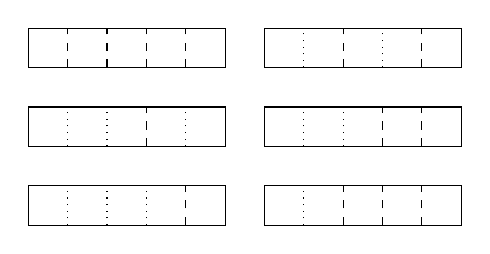
\begin{tikzpicture}[scale = 0.5]
						\draw (0,0)rectangle++(5,1);
						\foreach \x in {0,1,2,3,4,5}{
								\draw [dashed](0,0)++(\x,0)--(\x,1);
							}

						\draw (6,0)rectangle++(5,1);
						\foreach \x in {0,1,3,5}{
								\draw [dotted](6,0)++(\x,0)--++(0,1);
							}
						\draw [dashed](6,0)++(2,0)--++(0,1);
						\draw [dashed](6,0)++(4,0)--++(0,1);




						\draw (0,-2)rectangle++(5,1);
						\foreach \x in {0,1,2,4,5}{
								\draw [dotted](0,-2)++(\x,0)--++(0,1);
							}
						\draw [dashed](0,-2)++(3,0)--++(0,1);

						\draw (6,-2)rectangle++(5,1);
						\foreach \x in {0,1,2,5}{
								\draw [dotted](6,-2)++(\x,0)--++(0,1);
							}
						\draw [dashed](6,-2)++(3,0)--++(0,1);
						\draw [dashed](6,-2)++(4,0)--++(0,1);





						\draw (0,-4)rectangle++(5,1);
						\foreach \x in {0,1,2,3,5}{
								\draw [dotted](0,-4)++(\x,0)--++(0,1);
							}

						\draw [dashed](0,-4)++(4,0)--++(0,1);
						\draw (6,-4)rectangle++(5,1);
						\foreach \x in {0,1}{
								\draw [dotted](6,-4)++(\x,0)--++(0,1);
							}
						\draw [dashed](6,-4)++(4,0)--++(0,1);
						\draw [dashed](6,-4)++(3,0)--++(0,1);
						\draw [dashed](6,-4)++(2,0)--++(0,1);

					\end{tikzpicture}
				 \end{center}
			}
			\\
			\midrule
			\makecell{7                  \\ 1 4 10 8 5 10 13} & 21 & In questo caso ciò che conviene fare è spezzare il cilindro in 2 pezzi di lunghezza 3 e 1 di lunghezza 1:
			{
			\begin{center}
				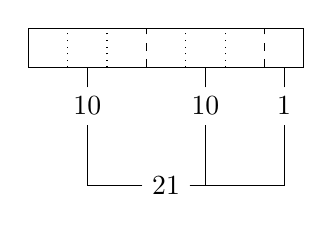
\begin{tikzpicture}[scale = 0.5]
					\draw (0,0)rectangle++(7,1);
					\foreach \x in {0,1,2,4,5,7}{
							\draw [dotted](0,0)++(\x,0)--(\x,1);
						}
					\draw [dashed](3,0)--++(0,1);
					\draw [dashed](6,0)--++(0,1);

					\node (a)[anchor = north] at(1.5, -0.5)  {10};
					\node (b)[anchor = north] at(4.5, -0.5)  {10};
					\node (c)[anchor = north] at(6.5, -0.5)  {1};
					\draw (a.north)--++(0,0.5);
					\draw (b.north)--++(0,0.5);
					\draw (c.north)--++(0,0.5);

					\node (d)at(3.5, -3)  {21};
					\draw (d)-|(a);
					\draw (d)-|(b);
					\draw (d)-|(c);
				\end{tikzpicture}
			\end{center}
			}
			\\
			\bottomrule
		\end{tabularx}
	\end{center}
	\tikzexternalenable

	Complessità ottimale: $ O\left(n \cdot v.size\left(\right)\right) $
\end{esercizio}\label{cuttingrod}

L'idea di base per risolvere il problema è la seguente:
\begin{itemize}
	\item Creo un vettore \verb|dp| all'interno del quale salvo \underline{nella $ i $-\textit{esima} cella il valore massimo che posso ottenere suddividendo un cilindro di lunghezza $ i+1 $}
	\item Costruisco il vettore \verb|dp| partendo dal caso base: \verb|dp[0] = prezzi [0]|, in quanto ho un solo modo di suddividere un cilindro lungo 1
	\item Contanto sul fatto che il vettore \verb|dp| contenga il \underline{il prezzo maggiore che posso ottenere suddividendo il cilindro in un dato modo}, calcolo \verb|dp[i+1]| sfruttando i dati contenuti nelle celle precedenti del vettore \verb|dp|.In particolare, supponendo di dover calcolare la posizione $ i $ del vettore \verb|dp|, devo:
	      \begin{itemize}
		      \item Calcolare il prezzo che otterrei mettendo in posizione $ i $ un pezzo di ogni lunghezza, da 1 a $ i $
		      \item Confrontare i prezzi ottenuti
		      \item \verb|dp[i]| è il valore massimo fra questi prezzi
	      \end{itemize}
\end{itemize}
Vediamo un esempio grafico. Supponiamo di avere in input il vettore \verb|prezzi|, con valori:
\begin{center}
	1 4 10 8 5 10 13
\end{center}
Ripercorriamo gli step appena descritti.

\begin{itemize}
	\item Creo un vettore \verb|dp| all'interno del quale salvo \underline{nella $ i $-\textit{esima} cella il valore massimo che posso ottenere suddividendo un cilindro di lunghezza $ i+1 $}
	\item Costruisco il vettore \verb|dp| partendo dal caso base: \verb|dp[0] = prezzi [0]|, in quanto ho un solo modo di suddividere un cilindro lungo 1. Quindi nel nostro caso:

	      \begin{center}
		      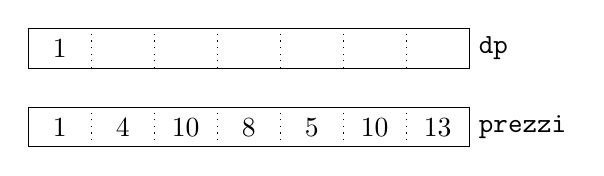
\begin{tikzpicture}[yscale = 0.5, xscale = 0.8]
			      \draw (0,-2)rectangle++(7,1);
			      \foreach \x in {0,1,2,3,4,5,6,7}{
					      \draw [dotted](0,-2)++(\x,0)--++(0,1);
				      }
			      \node  at (0.5,-1.5)  {1};
			      \node  at (1.5,-1.5)  {4};
			      \node  at (2.5,-1.5)  {10};
			      \node  at (3.5,-1.5)  {8};
			      \node  at (4.5,-1.5)  {5};
			      \node  at (5.5,-1.5)  {10};
			      \node  at (6.5,-1.5)  {13};

			      \node  [anchor = west] at (7,-1.5)  {\ttfamily prezzi};


			      \draw (0,0)rectangle++(7,1);
			      \foreach \x in {0,1,2,3,4,5,6,7}{
					      \draw [dotted](0,0)++(\x,0)--(\x,1);
				      }
			      \node  at (0.5,0.5)  {1};
			      \node  [anchor = west] at (7,0.5)  {\ttfamily dp};

		      \end{tikzpicture}
	      \end{center}

	      Chiaramente, un cilindro id lunghezza 1 non può essere suddiviso, quindi l'unico prezzo possibile è il prezzo del cilindro lungo 1, ossia 1 nel nostro caso


	\item Contanto sul fatto che il vettore \verb|dp| contenga il \underline{il prezzo maggiore che posso ottenere suddividendo il cilindro in un dato modo}, calcolo \verb|dp[i+1]| sfruttando i dati contenuti nelle celle precedenti del vettore \verb|dp|.In particolare, supponendo di dover calcolare la posizione $ i $ del vettore \verb|dp|, devo:
	      \begin{itemize}
		      \item Calcolare il prezzo che otterrei mettendo in posizione $ i $ un pezzo di ogni lunghezza, da 1 a $ i $
		      \item Confrontare i prezzi ottenuti
		      \item \verb|dp[i]| è il valore massimo fra questi prezzi
	      \end{itemize}
	      Iniziamo quindi calcolando \verb|v[1]|. So di avere già calcolato il prezzo migliore per suddividere un cilindro di lunghezza $ 1 $. Quindi per arrivare ad avere un cilindro di lunghezza 2 ho due alternative:

	      \begin{center}
		      \begin{tikzpicture}[yscale = 0.5, xscale = 1.3]


			      \draw (0,2)rectangle++(2,2);
			      \draw (0,3)--(2,3);

			      \node ()[anchor = west]at (2,3.5) {Aggiungo pezzo lungo 1};
			      \node ()[anchor = west]at (2,2.5) {Aggiungo pezzo lungo 2};

			      \draw [pattern = north east lines](1,3)rectangle(2,4);
			      \draw [pattern = north east lines](0,2)rectangle(2,3);

			      \node () at (0.5,3.5)  {\ttfamily dp[0]};
			      \node () at (1.5,3.5)  {\contour{white}{1}};

			      \node () at (1, 2.5)  {\contour{white}{4}};

		      \end{tikzpicture}
	      \end{center}
	      Ora devo decidere se mi convenga prendere un solo cilindro da 2 oppure suddividerlo in due pezzi da 1. Mi basta però vedere quale delle opzioni ha prezzo maggiore. In questo caso conviene prendere un pezzo da 2 con costo 4. Dp diventa:

	      \begin{center}
		      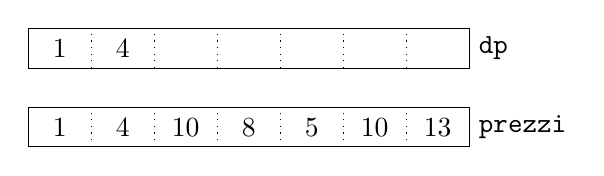
\begin{tikzpicture}[yscale = 0.5, xscale = 0.8]
			      \draw (0,0)rectangle++(7,1);
			      \foreach \x in {0,1,2,3,4,5,6,7}{
					      \draw [dotted](0,0)++(\x,0)--(\x,1);
				      }


			      \node  at (0.5,0.5)  {1};
			      \node  at (1.5,0.5)  {4};
			      \node  [anchor = west] at (7,0.5)  {\ttfamily dp};

			      \draw (0,-2)rectangle++(7,1);
			      \foreach \x in {0,1,2,3,4,5,6,7}{
					      \draw [dotted](0,-2)++(\x,0)--++(0,1);
				      }
			      \node  at (0.5,-1.5)  {1};
			      \node  at (1.5,-1.5)  {4};
			      \node  at (2.5,-1.5)  {10};
			      \node  at (3.5,-1.5)  {8};
			      \node  at (4.5,-1.5)  {5};
			      \node  at (5.5,-1.5)  {10};
			      \node  at (6.5,-1.5)  {13};

			      \node  [anchor = west] at (7,-1.5)  {\ttfamily prezzi};

		      \end{tikzpicture}
	      \end{center}

	      Ripetiamo il passaggio per $ i=3 $
\end{itemize}

\newcommand{\dpvector}{
	\def\rows{1}
	\def\columns{7}
	\def\shiftx{0}
	\def\shifty{-2}


	\foreach \x in {0,1,...,\columns}{
			\draw [dotted](0 + \shiftx,0 + \shifty)++(\x,0)--++(0,\rows);
		}

	\draw (\shiftx, \shifty)rectangle++(\columns, \rows);

	\node ()[anchor = west]at(7,-1.5) {\ttfamily dp};
}

\begin{minipage}[t]{0.48\textwidth}
	\begin{tikzpicture}[yscale = 0.5, xscale = 1.3]


		\def\rows{3}
		\def\columns{3}
		\newcommand{\shiftx}{0}
		\newcommand{\shifty}{0}


		\foreach \x in {0,1,...,\columns}{
				\draw [dotted](0 + \shiftx,0 + \shifty)++(\x,0)--++(0,\rows);
			}

		\foreach \x in {0,1,...,\rows}{
				\draw (0 + \shiftx,0 + \shifty)++(0,\x)--++(\columns,0);
			}

		\draw (\shiftx, \shifty)rectangle++(\columns, \rows);


		\foreach \x in {\rows,...,1}{
				\draw [pattern = north east lines](\shiftx + \columns - \x,\shifty + \rows - \x)rectangle++(\x, );
			}


		\node ()at (2.5, 2.5)  {\contour{white}{1}};
		\node ()at (2, 1.5)  {\contour{white}{4}};
		\node ()at (1.5, 0.5)  {\contour{white}{10}};

		\node ()at(1.5,2.5)  {\ttfamily dp[1]};
		\node ()at(0.5,1.5)  {\ttfamily dp[0]};




	\end{tikzpicture}
	\vskip3mm
	\begin{tikzpicture}[yscale = 0.5, xscale = 0.8]

		\dpvector

		\node ()at(0.5,-1.5) {1};
		\node ()at(1.5,-1.5) {4};
		\node ()at(2.5,-1.5) {\textcolor{gray}{10}};
	\end{tikzpicture}
\end{minipage}
%
\begin{minipage}[t]{0.48\textwidth}

	\begin{tikzpicture}[yscale = 0.5, xscale = 1.3]
		\def\rows{4}
		\def\columns{4}
		\newcommand{\shiftx}{0}
		\newcommand{\shifty}{0}


		\foreach \x in {0,1,...,\columns}{
				\draw [dotted](0 + \shiftx,0 + \shifty)++(\x,0)--++(0,\rows);
			}

		\foreach \x in {0,1,...,\rows}{
				\draw (0 + \shiftx,0 + \shifty)++(0,\x)--++(\columns,0);
			}

		\draw (\shiftx, \shifty)rectangle++(\columns, \rows);


		\foreach \x in {\rows,...,1}{
				\draw [pattern = north east lines](\shiftx + \columns - \x,\shifty + \rows - \x)rectangle++(\x, );
			}

		\node ()at (3.5, 3.5)  {\contour{white}{1}};
		\node ()at (3, 2.5)  {\contour{white}{4}};
		\node ()at (2.5, 1.5)  {\contour{white}{10}};
		\node ()at (2, 0.5)  {\contour{white}{8}};

		\node ()at(2.5,3.5)  {\ttfamily dp[2]};
		\node ()at(1.5,2.5)  {\ttfamily dp[1]};
		\node ()at(0.5,1.5)  {\ttfamily dp[0]};
	\end{tikzpicture}
	\vskip3mm
	\begin{tikzpicture}[yscale = 0.5, xscale = 0.8]

		\dpvector

		\node ()at(0.5,-1.5) {1};
		\node ()at(1.5,-1.5) {4};
		\node ()at(2.5,-1.5) {10};
		\node ()at(3.5,-1.5) {\textcolor{gray}{11}};
	\end{tikzpicture}
\end{minipage}


\vskip20mm


%
\begin{minipage}[t]{0.48\textwidth}
	\begin{tikzpicture}[yscale = 0.5, xscale = 1.3]
		\def\rows{5}
		\def\columns{5}
		\newcommand{\shiftx}{0}
		\newcommand{\shifty}{0}


		\foreach \x in {0,1,...,\columns}{
				\draw [dotted](0 + \shiftx,0 + \shifty)++(\x,0)--++(0,\rows);
			}

		\foreach \x in {0,1,...,\rows}{
				\draw (0 + \shiftx,0 + \shifty)++(0,\x)--++(\columns,0);
			}

		\draw (\shiftx, \shifty)rectangle++(\columns, \rows);


		\foreach \x in {\rows,...,1}{
				\draw [pattern = north east lines](\shiftx + \columns - \x,\shifty + \rows - \x)rectangle++(\x, );
			}

		\node ()at (4.5, 4.5)  {\contour{white}{1}};
		\node ()at (4, 3.5)  {\contour{white}{4}};
		\node ()at (3.5, 2.5)  {\contour{white}{10}};
		\node ()at (3, 1.5)  {\contour{white}{8}};
		\node ()at (2.5, 0.5)  {\contour{white}{5}};

		\node ()at(3.5,4.5)  {\ttfamily dp[3]};
		\node ()at(2.5,3.5)  {\ttfamily dp[2]};
		\node ()at(1.5,2.5)  {\ttfamily dp[1]};
		\node ()at(0.5,1.5)  {\ttfamily dp[0]};
	\end{tikzpicture}
	\vskip3mm
	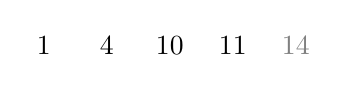
\begin{tikzpicture}[yscale = 0.5, xscale = 0.8]

		\dpvector

		\node ()at(0.5,-1.5) {1};
		\node ()at(1.5,-1.5) {4};
		\node ()at(2.5,-1.5) {10};
		\node ()at(3.5,-1.5) {11};
		\node ()at(4.5,-1.5) {\textcolor{gray}{14}};
	\end{tikzpicture}
\end{minipage}
%
\begin{minipage}[t]{0.48\textwidth}
	\begin{tikzpicture}[yscale = 0.5, xscale = 1.3]
		\def\rows{6}
		\def\columns{6}
		\newcommand{\shiftx}{0}
		\newcommand{\shifty}{0}


		\foreach \x in {0,1,...,\columns}{
				\draw [dotted](0 + \shiftx,0 + \shifty)++(\x,0)--++(0,\rows);
			}

		\foreach \x in {0,1,...,\rows}{
				\draw (0 + \shiftx,0 + \shifty)++(0,\x)--++(\columns,0);
			}

		\draw (\shiftx, \shifty)rectangle++(\columns, \rows);


		\foreach \x in {\rows,...,1}{
				\draw [pattern = north east lines](\shiftx + \columns - \x,\shifty + \rows - \x)rectangle++(\x, );
			}

		\node ()at (5.5, 5.5)  {\contour{white}{1}};
		\node ()at (5, 4.5)  {\contour{white}{4}};
		\node ()at (4.5, 3.5)  {\contour{white}{10}};
		\node ()at (4, 2.5)  {\contour{white}{8}};
		\node ()at (3.5, 1.5)  {\contour{white}{5}};
		\node ()at (3, 0.5)  {\contour{white}{10}};

		\node ()at(4.5,5.5)  {\ttfamily dp[4]};
		\node ()at(3.5,4.5)  {\ttfamily dp[3]};
		\node ()at(2.5,3.5)  {\ttfamily dp[2]};
		\node ()at(1.5,2.5)  {\ttfamily dp[1]};
		\node ()at(0.5,1.5)  {\ttfamily dp[0]};
	\end{tikzpicture}
	\vskip3mm
	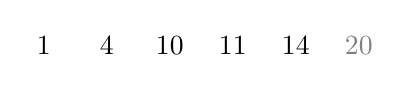
\begin{tikzpicture}[yscale = 0.5, xscale = 0.8]

		\dpvector

		\node ()at(0.5,-1.5) {1};
		\node ()at(1.5,-1.5) {4};
		\node ()at(2.5,-1.5) {10};
		\node ()at(3.5,-1.5) {11};
		\node ()at(4.5,-1.5) {14};
		\node ()at(5.5,-1.5) {\textcolor{gray}{20}};
	\end{tikzpicture}

\end{minipage}

\vskip15mm

\begin{tikzpicture}[yscale = 0.5, xscale = 1.3]
	\def\rows{7}
	\def\columns{7}
	\newcommand{\shiftx}{0}
	\newcommand{\shifty}{0}


	\foreach \x in {0,1,...,\columns}{
			\draw [dotted](0 + \shiftx,0 + \shifty)++(\x,0)--++(0,\rows);
		}

	\foreach \x in {0,1,...,\rows}{
			\draw (0 + \shiftx,0 + \shifty)++(0,\x)--++(\columns,0);
		}

	\draw (\shiftx, \shifty)rectangle++(\columns, \rows);


	\foreach \x in {\rows,...,1}{
			\draw [pattern = north east lines](\shiftx + \columns - \x,\shifty + \rows - \x)rectangle++(\x, );
		}

	\node ()at (6.5, 6.5)  {\contour{white}{1}};
	\node ()at (6, 5.5)  {\contour{white}{1}};
	\node ()at (5.5, 4.5)  {\contour{white}{4}};
	\node ()at (5, 3.5)  {\contour{white}{10}};
	\node ()at (4.5, 2.5)  {\contour{white}{8}};
	\node ()at (4, 1.5)  {\contour{white}{5}};
	\node ()at (3.5, 0.5)  {\contour{white}{10}};

	\node ()at(5.5,6.5)  {\ttfamily dp[5]};
	\node ()at(4.5,5.5)  {\ttfamily dp[4]};
	\node ()at(3.5,4.5)  {\ttfamily dp[3]};
	\node ()at(2.5,3.5)  {\ttfamily dp[2]};
	\node ()at(1.5,2.5)  {\ttfamily dp[1]};
	\node ()at(0.5,1.5)  {\ttfamily dp[0]};
\end{tikzpicture}
\vskip3mm
\begin{tikzpicture}[yscale = 0.5, xscale = 1.3]

	\dpvector

	\node ()at(0.5,-1.5) {1};
	\node ()at(1.5,-1.5) {4};
	\node ()at(2.5,-1.5) {10};
	\node ()at(3.5,-1.5) {11};
	\node ()at(4.5,-1.5) {14};
	\node ()at(5.5,-1.5) {20};
	\node ()at(6.5,-1.5) {\textcolor{gray}{21}};
\end{tikzpicture}


\begin{esercizio}{Somma e media \href{https://training.olinfo.it/\#/task/array/statement}{(link)}}
	Dati in input un numero $ N $, e successivamente $ N $ interi, calcolare la media aritmetica e la somma di questi ultimi
	\vskip3mm
	\underline{Input:}
	\vskip3mm Sulla prima riga l'intero $ N $, sulla seconda riga $ N $ interi separati da uno spazio
	\vskip3mm
	\underline{Output:}
	\vskip3mm Due interi: rispettivamente la somma degli $ N $ numeri e la loro media aritmetica
	\renewcommand{\cellalign}{l}
	\vskip3mm
	\begin{tabularx}{\textwidth}{llX}
		\toprule
		Input & Output & Discussione \\
		\midrule
		\makecell{1                  \\ 12} & 12 12 & Somma e media coincidono e hanno valore 12\\[12pt]
		\makecell{7                  \\ 1 2 34 -56 33 23 89} & 126 18 & Somma e media coincidono e hanno valore 12\\
		\bottomrule
	\end{tabularx}
	\vskip3mm
	Complessità ottimale: $ O\left(N\right) $
\end{esercizio}

\begin{esercizio}{Majority element \href{https://leetcode.com/problems/majority-element/submissions/}{(link)}}
	Dato un array \textit{nums} di dimentione $ n $, ritornare il \textit{majority element}. Il \textit{majority element} è l'elemento che appare \underline{di più} di $ \frac{n}{2} $ volte. Si può assumere che l'elemento esista sempre nell'array
	\vskip3mm
	\underline{Input:}
	\vskip3mm Sulla prima riga l'intero $ n $, sulla seconda riga $ n $, ossia gli elementi di \textit{nums}
	\vskip3mm
	\underline{Output:}
	\vskip3mm Un intero, il majority element
	\vskip3mm
	\renewcommand{\cellalign}{l}
	\begin{tabularx}{\textwidth}{llX}
		\toprule
		Input & Output & Discussione \\
		\midrule
		\makecell{3                  \\ 3 2 3} & 3 & 3 appare più di 3/2 = 1 volta \\[12pt]
		\makecell{7                  \\ 2 2 1 1 1 2 2} & 2 & 2 appare più di 7/2 = 3 volte\\
		\bottomrule
	\end{tabularx}
	\vskip3mm
	Complessità ottimale: $ O\left(n\right) $
\end{esercizio}

\begin{esercizio}{Longest Common Subsequence \href{https://leetcode.com/problems/longest-common-subsequence/}{(link)}}
	Date in input due stringhe \textit{S1} ed \textit{S2}, si ritorni la lunghezza della \textit{longhest common subsequence}, ossia della \footnote{Con \underline{sottoseuquenza} si intende la una stringa che si può ottenere da un'altra eliminando determinati caratteri: \textit{bedbreakfast} è una sottosequenza di \textit{bedandbreakfast}. A differenza di ciò che accade in un \underline{sottovettore}, i caratteri \underline{non} devono essere necessariamente contigui: \textit{bedbreakfast} è sottosequenza ma non sottovettore; \textit{breakfast} è sottosequenza e sottovettore}{sottosequenza} più lunga comunque ad esntrambe le stringhe.
	\vskip3mm
	\underline{Input:}
	\vskip3mm Due stringhe, una per riga, composte da caratteri maiuscoli compresi fra $ A $ e $ Z $
	\vskip3mm
	\underline{Output:}
	\vskip3mm Un intero, la lunghezza della più lunga sottosequenza comune ad entrambe le stringhe
	\vskip3mm
	\renewcommand{\cellalign}{l}
	\begin{tabularx}{\textwidth}{llX}
		\toprule
		Input & Output & Discussione \\
		\midrule
		\makecell{AGGTAB             \\GXTXAYB} & 4 & La sottosequenza comune con lunghezza maggiore è \textit{"GTAB"}, ed ha lunghezza pari a 4  \\[12pt]
		\makecell{AABBCCD            \\  AABBD} & 5 & La sottosequenza comune con lunghezza maggiore è \textit{"AABBD", ed ha lunghezza pari a 5}\\
		\bottomrule
	\end{tabularx}
	\vskip3mm
	Complessità ottimale: $ O\left(s_1.lenght \cdot s_2.lenght\right) $
\end{esercizio}
Per risolvere questo problema dobbiamo utilizzare una matrice di supporto, che salverà i valori intermedi e ci permetterà di utilizzare la programmazione dinamica. Prendiamo come esempio il le stringhe \textit{"AGGTAB"} e \textit{"GXTXAYB"}. La matrice di supporto deve avere la seguente forma:
\begin{center}
	\begin{tabular}{cccccccccl}
		                          &                        & G                      & X                      & T                      & X                      & A                      & Y                      & B                      & s1, j \\ \cline{2-9}
		\multicolumn{1}{c|}{}     & \multicolumn{1}{c|}{0} & \multicolumn{1}{c|}{0} & \multicolumn{1}{c|}{0} & \multicolumn{1}{c|}{0} & \multicolumn{1}{c|}{0} & \multicolumn{1}{c|}{0} & \multicolumn{1}{c|}{0} & \multicolumn{1}{c|}{0} &       \\ \cline{2-9}
		\multicolumn{1}{c|}{A}    & \multicolumn{1}{c|}{0} & \multicolumn{1}{c|}{}  & \multicolumn{1}{c|}{}  & \multicolumn{1}{c|}{}  & \multicolumn{1}{c|}{}  & \multicolumn{1}{c|}{}  & \multicolumn{1}{c|}{}  & \multicolumn{1}{c|}{}  &       \\ \cline{2-9}
		\multicolumn{1}{c|}{G}    & \multicolumn{1}{c|}{0} & \multicolumn{1}{c|}{}  & \multicolumn{1}{c|}{}  & \multicolumn{1}{c|}{}  & \multicolumn{1}{c|}{}  & \multicolumn{1}{c|}{}  & \multicolumn{1}{c|}{}  & \multicolumn{1}{c|}{}  &       \\ \cline{2-9}
		\multicolumn{1}{c|}{G}    & \multicolumn{1}{c|}{0} & \multicolumn{1}{c|}{}  & \multicolumn{1}{c|}{}  & \multicolumn{1}{c|}{}  & \multicolumn{1}{c|}{}  & \multicolumn{1}{c|}{}  & \multicolumn{1}{c|}{}  & \multicolumn{1}{c|}{}  &       \\ \cline{2-9}
		\multicolumn{1}{c|}{T}    & \multicolumn{1}{c|}{0} & \multicolumn{1}{c|}{}  & \multicolumn{1}{c|}{}  & \multicolumn{1}{c|}{}  & \multicolumn{1}{c|}{}  & \multicolumn{1}{c|}{}  & \multicolumn{1}{c|}{}  & \multicolumn{1}{c|}{}  &       \\ \cline{2-9}
		\multicolumn{1}{c|}{A}    & \multicolumn{1}{c|}{0} & \multicolumn{1}{c|}{}  & \multicolumn{1}{c|}{}  & \multicolumn{1}{c|}{}  & \multicolumn{1}{c|}{}  & \multicolumn{1}{c|}{}  & \multicolumn{1}{c|}{}  & \multicolumn{1}{c|}{}  &       \\ \cline{2-9}
		\multicolumn{1}{c|}{B}    & \multicolumn{1}{c|}{0} & \multicolumn{1}{c|}{}  & \multicolumn{1}{c|}{}  & \multicolumn{1}{c|}{}  & \multicolumn{1}{c|}{}  & \multicolumn{1}{c|}{}  & \multicolumn{1}{c|}{}  & \multicolumn{1}{c|}{}  &       \\ \cline{2-9}
		\multicolumn{1}{l}{s2, i} & \multicolumn{1}{l}{}   & \multicolumn{1}{l}{}   & \multicolumn{1}{l}{}   & \multicolumn{1}{l}{}   & \multicolumn{1}{l}{}   & \multicolumn{1}{l}{}   & \multicolumn{1}{l}{}   & \multicolumn{1}{l}{}   &
	\end{tabular}
\end{center}

Quindi la struttura della matrice è la seguente:
\begin{itemize}
	\item Un orentamento rappresenta una stringa, l'altro l'altra (nota che le stringhe non sono salvate nella matrice, sono riportate in figura solo per rendere il procedimento più chiaro)
	\item La prima colonna e la prima riga sono riempite di zeri. Questo serve perché ci permette di evitare di incappare in indici negativi quando eseguiremo l'algoritmo
	\item Siano \verb|s1| e \verb|s2| le stringhe, nella cella di indice $ \left(i,j\right) $, salveremo \underline{la lunghezza della longest common subsequence per {\ttfamily s1.substring(0,i)} e {\ttfamily s2.substring(0,j)}}
\end{itemize}
\vskip3mm
\begin{minipage}[c]{0.68\textwidth}
	\begin{center}
		\begin{tabular}{cccccccccl}
			                          &                        & G                      & X                      & T                      & X                      & A                      & Y                          & B                      & s1, j \\ \cline{2-9}
			\multicolumn{1}{c|}{}     & \multicolumn{1}{c|}{0} & \multicolumn{1}{c|}{0} & \multicolumn{1}{c|}{0} & \multicolumn{1}{c|}{0} & \multicolumn{1}{c|}{0} & \multicolumn{1}{c|}{0} & \multicolumn{1}{c|}{0}     & \multicolumn{1}{c|}{0} &       \\ \cline{2-9}
			\multicolumn{1}{c|}{A}    & \multicolumn{1}{c|}{0} & \multicolumn{1}{c|}{}  & \multicolumn{1}{c|}{}  & \multicolumn{1}{c|}{}  & \multicolumn{1}{c|}{}  & \multicolumn{1}{c|}{}  & \multicolumn{1}{c|}{}      & \multicolumn{1}{c|}{}  &       \\ \cline{2-9}
			\multicolumn{1}{c|}{G}    & \multicolumn{1}{c|}{0} & \multicolumn{1}{c|}{}  & \multicolumn{1}{c|}{}  & \multicolumn{1}{c|}{}  & \multicolumn{1}{c|}{}  & \multicolumn{1}{c|}{}  & \multicolumn{1}{c|}{(1,6)} & \multicolumn{1}{c|}{}  &       \\ \cline{2-9}
			\multicolumn{1}{c|}{G}    & \multicolumn{1}{c|}{0} & \multicolumn{1}{c|}{}  & \multicolumn{1}{c|}{}  & \multicolumn{1}{c|}{}  & \multicolumn{1}{c|}{}  & \multicolumn{1}{c|}{}  & \multicolumn{1}{c|}{}      & \multicolumn{1}{c|}{}  &       \\ \cline{2-9}
			\multicolumn{1}{c|}{T}    & \multicolumn{1}{c|}{0} & \multicolumn{1}{c|}{}  & \multicolumn{1}{c|}{}  & \multicolumn{1}{c|}{}  & \multicolumn{1}{c|}{}  & \multicolumn{1}{c|}{}  & \multicolumn{1}{c|}{}      & \multicolumn{1}{c|}{}  &       \\ \cline{2-9}
			\multicolumn{1}{c|}{A}    & \multicolumn{1}{c|}{0} & \multicolumn{1}{c|}{}  & \multicolumn{1}{c|}{}  & \multicolumn{1}{c|}{}  & \multicolumn{1}{c|}{}  & \multicolumn{1}{c|}{}  & \multicolumn{1}{c|}{}      & \multicolumn{1}{c|}{}  &       \\ \cline{2-9}
			\multicolumn{1}{c|}{B}    & \multicolumn{1}{c|}{0} & \multicolumn{1}{c|}{}  & \multicolumn{1}{c|}{}  & \multicolumn{1}{c|}{}  & \multicolumn{1}{c|}{}  & \multicolumn{1}{c|}{}  & \multicolumn{1}{c|}{}      & \multicolumn{1}{c|}{}  &       \\ \cline{2-9}
			\multicolumn{1}{l}{s2, i} & \multicolumn{1}{l}{}   & \multicolumn{1}{l}{}   & \multicolumn{1}{l}{}   & \multicolumn{1}{l}{}   & \multicolumn{1}{l}{}   & \multicolumn{1}{l}{}   & \multicolumn{1}{l}{}       & \multicolumn{1}{l}{}   &
		\end{tabular}
	\end{center}
\end{minipage}
%
\begin{minipage}[c]{0.30\textwidth}
	Ad esempio, nella cella evidenziata, con indice $ \left(1,6\right) $, va salvata la lunghezza della LCS delle stringhe "GXTXAY" e "AG"
\end{minipage}
\vskip3mm
Detto questo, possiamo riempire la tabella secondo i seguenti criteri:
\begin{itemize}
	\item Se {\ttfamily s1[i-1] == s2[j-1]} ciò significa che la soluzione ottimale per quel sottoproblema è data dalla soluzione ottimale per il sottoproblema con le medesime stringhe senza però questultimo carattere. La soluzione di questo problema si trova nella cella $ \left(i-2, j-2\right) $
	\item Se {\ttfamily s1[i-1] != s2[j-1]} allora non ho modo di migliorare la lunghezza della LCS aggiungendo un elemento alle sottostringhe dei problemi precedenti. La soluzione ottimale è quindi da calcolare confrontando le soluzioni ottimali precedenti, in particolare sia {\ttfamily dp} la matrice:
	      \begin{center}
		      \ttfamily dp[i][j] = Math.max(dp[i-1][j], dp[i][j-1])
	      \end{center}
	      Volendo ad esempio calcolare il problema per le sottostringhe "GXT" e "AGGTA" posso partire dalle soluzioni dei sottoproblemi per le stringhe "GX", "AGGTA" e "GXT", "AGGT". Mi basta prendere la maggiore di queste due.
	      \vskip3mm
	      Nota anche che non mi serve controllare la soluzione del sottoproblema "GX", "AGGT" in quanto colonne e righe sono tutte ordinate in maniera crescente, quindi è impossibile che la cella $ \left(i-1, j-1\right) $ abbia un valore maggiore della cella $ \left(i, j-1\right) $ o $ \left(i-1, j\right) $
\end{itemize}

\begin{esercizio}{Minimum coin \href{https://leetcode.com/problems/coin-change/description/}{(link)}}
	Vengono dati in input un array contenente un array {\ttfamily coins} (il quale rappresenta monete di diverso taglio) e un numero intero {\ttfamily ammount} (il quale rappresenta il quantitativo totale di monete). Calcolare il numero minimo di monete che si possono utilizzare per arrivare alla somma {\ttfamily ammount} . Si assuma di avere un numero infinito di monete per ogni taglio.
	\vskip3mm
	\underline{Input:}
	\vskip3mm Due righe. Sulla prima gli interi {\ttfamily ammount}  e {\ttfamily n}  (la dimensione di {\ttfamily coins} ), mentre sulla seconda gli elementi di {\ttfamily coins}  separati da uno spazio. Nota che gli elementi di {\ttfamily coins} non vengono necessariamente dati in ordine crescente
	\vskip3mm
	\underline{Output:}
	\vskip3mm Un intero, il numero minimo necessario di monete per arrivare ad {\ttfamily ammount}. Se la combinazione non fosse presente ritornare -1
	\vskip3mm
	\renewcommand{\cellalign}{l}
	\begin{tabularx}{\textwidth}{llX}
		\toprule
		Input & Output & Discussione \\
		\midrule
		\makecell{11 3               \\ 1 2 5} & 3 & Per ottenere la somma 11 posso utilizzare 2 monete da 5 e 1 da 1 \\[12pt]
		\makecell{4 1                \\  3} & -1 & Non è possibile ottenere una somma di 4 con sole monete da 3\\
		\bottomrule
	\end{tabularx}
	\vskip3mm
	Complessità ottimale: $ O\left(coins.size \cdot amount\right) $
\end{esercizio}
Approccio intuitivo (sbagliato): cerco di riempire la somma con monete quanto più grandi possibile. Ad esempio con questo input, tuttavia, non funziona: somma: 20, monete: 15 13 7 1
\vskip3mm
L'approccio corretto è molto simile al problema \textit{\hyperref[cuttingrod]{cutting rod}}. Di fatto è come se dovessimo "riempire" un cilindro lungo {\ttfamily ammount} con pezzi di dimensioni contenute in {\ttfamily coins}.
\vskip3mm
Procediamo così:
\begin{itemize}
	\item Creo vettore \verb|dp| di dimensione \verb|ammount|, all'interno del quale salvo nella cella $ i $ il numero minore di monete per creare una somma pari ad $ i $
	\item \verb|dp[0]=0|, ossia ho modo di creare una somma pari a zero con zero monete
	\item Per calcolare la cella i-esima del vettore \verb|dp|, devo ragionare nel seuguente modo:
	      \begin{itemize}
		      \item Per ogni moneta che abbbia valore inferiore a $ i $, calcoliamo il minor numero di monete che possiamo usare utilizzando il vettore \verb|dp|, in analogia con il problema \textit{\hyperref[cuttingrod]{cutting rod}}. Supponiamo di avere \verb|amount=5, coins=[1, 2, 3, 4]|
		            \begin{center}

			            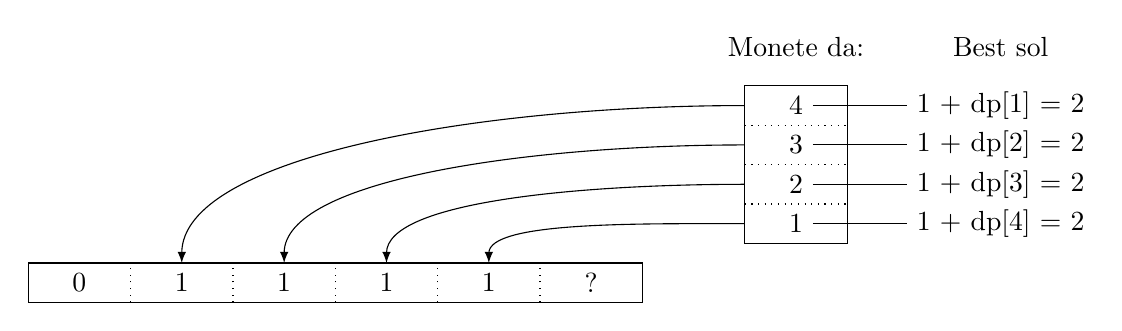
\begin{tikzpicture}[yscale = 0.5, xscale = 1.3]
				            \def\rows{1}
				            \def\columns{6}
				            \newcommand{\shiftx}{0}
				            \newcommand{\shifty}{0}


				            \foreach \x in {0,1,...,\columns}{
						            \draw [dotted](0 + \shiftx,0 + \shifty)++(\x,0)--++(0,\rows);
					            }

				            \foreach \x in {0,1,...,\rows}{
						            \draw (0 + \shiftx,0 + \shifty)++(0,\x)--++(\columns,0);
					            }

				            \draw (\shiftx, \shifty)rectangle++(\columns, \rows);

				            %\draw [-latex](5 - 0.5, 1)to[out=90, in=90](4 - 0.5, 1);
				            \node at (1 - 0.5, \shifty + 0.5) {0};
				            \node at (2 - 0.5, \shifty + 0.5) {1};
				            \node at (3 - 0.5, \shifty + 0.5) {1};
				            \node at (4 - 0.5, \shifty + 0.5) {1};
				            \node at (5 - 0.5, \shifty + 0.5) {1};
				            \node at (6 - 0.5, \shifty + 0.5) {?};

				            \draw (\columns + 1, 1.5)rectangle(\columns + 2, 5.5);

				            \foreach \x in {0,1,...,2}{
						            \draw [dotted](\columns + 1, 2.5 + \x)--++(1,0);
					            }

				            \node (a)at(\columns + 1.5, 2) {1};
				            \node (b)at(\columns + 1.5, 3) {2};
				            \node (c)at(\columns + 1.5, 4) {3};
				            \node (d)at(\columns + 1.5, 5) {4};
				            \node  at(\columns + 1.5, 6.5) {Monete da:};

				            \draw [-latex](\columns + 1, 5)to[out = 180, in=90](1.5, 1);
				            \draw [-latex](\columns + 1, 4)to[out = 180, in=90](2.5, 1);
				            \draw [-latex](\columns + 1, 3)to[out = 180, in=90](3.5, 1);
				            \draw [-latex](\columns + 1, 2)to[out = 180, in=90](4.5, 1);

				            \node (1)at(\columns + 3.5, 2) {1 + dp[4] = 2};
				            \node (2)at(\columns + 3.5, 3) {1 + dp[3] = 2};
				            \node (3)at(\columns + 3.5, 4) {1 + dp[2] = 2};
				            \node (4)at(\columns + 3.5, 5) {1 + dp[1] = 2};
				            \node  at(\columns + 3.5, 6.5) {Best sol};

				            \draw (a)--(1);
				            \draw (b)--(2);
				            \draw (c)--(3);
				            \draw (d)--(4);
			            \end{tikzpicture}

			            La miglior souzione per una somma pari a 5 è quindi 2. Possiamo usare 2 monete in modi diversi ((3,2), (4,1)) per ottenere la somma 5
		            \end{center}
	      \end{itemize}
	\item Mettendo in ordine il concetto intuitivo dobbiamo creare \verb|dp[i]| mettendo nel seguente modo:
	      \begin{itemize}
		      \item Per ogni elemento di \verb|coins| che sia minore di \verb|i| calcolo il numero minimo di monete che è necessario per arrivare ad una somma di \verb|i| utilizzando \verb|dp|. Supponendo di dover includere una moneta di valore \verb|value|, allora il minor numero di monete per arrivare a \verb|i| è dato da
		            \begin{center}
			            \verb|dp[i-value] + 1|
		            \end{center}
		      \item Il valore minimo di monete per arrivare alla somma \verb|i| è il valore minimo fra tutti quelli calcolari al punto precedente
		      \item Occhio ai casi nei quali non è possibile ottenere una somma specifica tramite le monete a disposizione. In questi casi metteremo il valore -1 nel vettore \verb|dp|
	      \end{itemize}
\end{itemize}
\begin{esercizio}{Unique paths \href{https://leetcode.com/problems/unique-paths/description/}{(link)} }
	Un robot si muove su di una griglia {\ttfamily n x m}. Il robot inizialmente è posizionato sulla cella $ \left[0\right]\left[0\right] $ e deve arrivare alla cella $ \left[m-1\right]\left[n-1\right] $. Il robot può muoversi solamente verso il basso e verso destra. Dati due interi {\ttfamily n, m} che indicano la dimensione della griglia, calcolare il numero di percosi possibili
	\vskip3mm
	\vskip3mm
	\underline{Input}
	\vskip3mm
	Gli interi {\ttfamily m} e {\ttfamily n}
	\vskip3mm
	\underline{Output}
	\vskip3mm
	Il numero di percorsi possibili
	\renewcommand{\cellalign}{l}
	\begin{center}
		\begin{tabularx}{\textwidth}{llX}
			\toprule
			Input & Output & Discussione                                                                                        \\
			\midrule
			2 2   & 2      & I percorsi possibili sono $[(R \rightarrow D), (D \rightarrow R)]$                                 \\[12pt]
			3 2   & 3      & I percorsi possibili sono \vskip0mm
			$(R \rightarrow D \rightarrow D)$, $(D \rightarrow D \rightarrow R)$, $\left(D \rightarrow R \rightarrow D\right)]$ \\
			\bottomrule
		\end{tabularx}
	\end{center}
	Complessità ottimale: $ O\left(n \cdot  m\right) $
\end{esercizio}\label{uniquepaths}

L'idea di base è la seguente:
\begin{itemize}
	\item Creo matrice {\ttfamily dp} che salva nella generica cella $ \left[i\right]\left[j\right] $ il numero di percorsi tramite i quali posso arrivare in $ \left[i\right]\left[j\right] $
	\item Inizializzo la prima colonna e la prima riga della matrice a 1: per raggiungere le celle della prima riga e colonna ho un solo modo, ossia rispettivamente spostarmi a destra o spostarmi in basso (non posso tornare indietro)
	\item Per ogni cella che avanza calcolo il valore come la somma della cella a sinistra e della cella a sopra: questo perche per arrivare nella cella $ \left[i\right]\left[j\right] $ posso passare per la cella $ \left[i-1\right]\left[j\right] $ oppure per la cella $ \left[i\right]\left[j-1\right] $. La somma dei modi che ho per arrivare nelle suddette celle è il numero di modi che ho per arrivare nella cella corrente
	\item Una volta generata l'intera tabella, nella ultima cella in basso a destra avro il risultato al problema
\end{itemize}
\begin{gather*}
	\begin{bmatrix}
		1 & 1 & 1 & 1 & 1 & 1 & 1 \\
		1 & 2 & / & / & / & / & / \\
		1 & / & / & / & / & / & / \\
	\end{bmatrix}
	\begin{bmatrix}
		1 & 1 & 1 & 1 & 1 & 1 & 1 \\
		1 & 2 & 3 & / & / & / & / \\
		1 & / & / & / & / & / & / \\
	\end{bmatrix}
	\begin{bmatrix}
		1 & 1 & 1 & 1 & 1 & 1 & 1 \\
		1 & 2 & 3 & 4 & / & / & / \\
		1 & / & / & / & / & / & / \\
	\end{bmatrix}
	\begin{bmatrix}
		1 & 1 & 1 & 1 & 1 & 1 & 1 \\
		1 & 2 & 3 & 4 & 5 & / & / \\
		1 & / & / & / & / & / & / \\
	\end{bmatrix}
	\\
	\begin{bmatrix}
		1 & 1 & 1 & 1 & 1 & 1 & 1 \\
		1 & 2 & 3 & 4 & 5 & 6 & / \\
		1 & / & / & / & / & / & / \\
	\end{bmatrix}
	\begin{bmatrix}
		1 & 1 & 1 & 1 & 1 & 1 & 1 \\
		1 & 2 & 3 & 4 & 5 & 6 & 7 \\
		1 & / & / & / & / & / & / \\
	\end{bmatrix}
	\begin{bmatrix}
		1 & 1 & 1 & 1 & 1 & 1 & 1 \\
		1 & 2 & / & / & / & / & / \\
		1 & 3 & / & / & / & / & / \\
	\end{bmatrix}
	\begin{bmatrix}
		1 & 1 & 1 & 1 & 1 & 1 & 1 \\
		1 & 2 & 3 & / & / & / & / \\
		1 & 3 & 6 & / & / & / & / \\
	\end{bmatrix}
	\\
	\begin{bmatrix}
		1 & 1 & 1 & 1  & 1 & 1 & 1 \\
		1 & 2 & 3 & 4  & / & / & / \\
		1 & 3 & 6 & 10 & / & / & / \\
	\end{bmatrix}
	\begin{bmatrix}
		1 & 1 & 1 & 1  & 1  & 1 & 1 \\
		1 & 2 & 3 & 4  & 5  & / & / \\
		1 & 3 & 6 & 10 & 15 & / & / \\
	\end{bmatrix}
	\\
	\begin{bmatrix}
		1 & 1 & 1 & 1  & 1  & 1  & 1 \\
		1 & 2 & 3 & 4  & 5  & 6  & / \\
		1 & 3 & 6 & 10 & 15 & 21 & / \\
	\end{bmatrix}
	\begin{bmatrix}
		1 & 1 & 1 & 1  & 1  & 1  & 1  \\
		1 & 2 & 3 & 4  & 5  & 6  & 7  \\
		1 & 3 & 6 & 10 & 15 & 21 & 28 \\
	\end{bmatrix}
\end{gather*}


\begin{esercizio}{Unique paths II \href{https://leetcode.com/problems/unique-paths/description/}{(link)} }
	Un robot si muove su di una griglia {\ttfamily n x m}. Il robot inizialmente è posizionato sulla cella $ \left[0\right]\left[0\right] $ e deve arrivare alla cella $ \left[m-1\right]\left[n-1\right] $. Il robot può muoversi solamente verso il basso e verso destra. Sulla griglia possono essere presenti degli ostacoli attraverso i quali il robot non può passare. Data una matrice {\ttfamily obstacles}, nella quale le celle con valore 1 indicano le celle con ostacoli, trovare il numero di percorsi possibili per arrivare nell'ultima cella in fondo a destra
	\vskip3mm
	\vskip3mm
	\underline{Input}
	\vskip3mm
	Gli interi {\ttfamily m} e {\ttfamily n} e nelle {\ttfamily m} righe successiva gli elementi della matrice {\ttfamily obstacles}
	\vskip3mm
	\underline{Output}
	\vskip3mm
	Il numero di percorsi possibili
	\renewcommand{\cellalign}{l}
	\begin{center}
		\begin{tabularx}{\textwidth}{llX}
			\toprule
			Input & Output & Discussione                                                                     \\
			\midrule
			\makecell{3 3                                                                                    \\ 0 0 0 \\ 0 1 0 \\ 0 0 0}& 2  & I percorsi possibili sono \vskip0mm
			$[(R \rightarrow R \rightarrow D \rightarrow D), (D \rightarrow D \rightarrow R \rightarrow R)]$ \\
			\bottomrule
		\end{tabularx}
	\end{center}
	Complessità ottimale: $ O\left(n \cdot  m\right) $
\end{esercizio}

L'idea è molto simile al problema \hyperref[uniquepaths]{Unique paths}, con l'unica differenza che dobbiamo tenere in considerazione i casi in cui una rotta è preclusa da un ostacolo. Inoltre, anzichè creare una nuova matrice {\ttfamily dp}, possiamo usare direttamente la matrice {\ttfamily obstacles} che ci viene data.
\begin{itemize}
	\item Riempio la prima colonna e riga della matrice {\ttfamily obstacles} con valore 1 fino al primo ostacolo. Dal primo ostacolo in poi avrò solo celle irraggiungibili. Setto le celle irraggiungibili con valore -1, in quanto usando 1 rischierei di confondere le celle irraggiungibili con le celle raggiungibili da 1 solo cammino
	\item Calcolo le celle rimanenti con la stessa logica usata in \hyperref[uniquepaths]{Unique paths}, tenendo conto però che:
	      \begin{itemize}
		      \item Nel caso ci sia un ostacolo nella cella a sinistra o in alto a quella corrente non posso arrivare da quella direzione. Se non rimane nemmeno una rotta possibile posso impostare il valore della della a -1, in quanto non riesco a ragiungerla in nessun modo
		      \item Nel caso ci sia un ostacolo nella cella corrente ({\ttfamily obstacles[i][j] == 1}) cambio il valore e metto -1, onde evitare ambiguità come spiegato precedentemente
	      \end{itemize}
	\item Ancora una volta, nella cella $ \left[m-1,n-1\right] $ ci sarà la soluzione del problema
\end{itemize}

\begin{gather*}
	\begin{bmatrix}
		0 & 0 & 0 \\
		0 & 1 & 0 \\
		0 & 0 & 0 \\
	\end{bmatrix}
	\xrightarrow{\text{riempio prima riga e colonna}}
	\begin{bmatrix}
		1 & 1 & 1 \\
		1 & 1 & 0 \\
		1 & 0 & 0 \\
	\end{bmatrix}
	\xrightarrow{\text{ cambio ostacolo in -1}}
	\begin{bmatrix}
		1 & 1  & 1 \\
		1 & -1 & 0 \\
		1 & 0  & 0 \\
	\end{bmatrix}
	\\
	\begin{bmatrix}
		1 & 1  & 1 \\
		1 & -1 & 1 \\
		1 & 0  & 0 \\
	\end{bmatrix}
	\begin{bmatrix}
		1 & 1  & 1 \\
		1 & -1 & 0 \\
		1 & 1  & 0 \\
	\end{bmatrix}
	\begin{bmatrix}
		1 & 1  & 1 \\
		1 & -1 & 1 \\
		1 & 1  & 2 \\
	\end{bmatrix}
\end{gather*}

\section{Feature importanti di cpp}
Di seguito vediamo una scarrellata di feature un filo più avanzate di c++ e della standard library che possono tornare molto utili in programmazione competitiva.
\subsection{Type inference - auto}\label{type inference}
Spesso con l'aumentare della complessità delle strutture dati, il tipo di una variabile può diventare molto lungo e difficile da scrivere. Per ovviare a questo problema, C++ fornisce la keyword \texttt{auto}, che permette al compilatore di dedurre automaticamente il tipo della variabile in fase di compilazione. Ad esempio, per inizializzare un iteratore, anzichè scrivere:
\begin{center}
	\ttfamily
	std::vector<int>::iterator it = vec.begin();
\end{center}
possiamo scrivere:
\begin{center}
	\ttfamily
	auto it = vec.begin();
\end{center}
Questo meccanisco si chiama \textit{type inference}. Di fatto affidiamo al compilatore il compito di dedurre il tipo della variabile in base al contesto

\subsection{Passaggio per riferimento}\label{pass by ref}
Solitamente in C++ le variabili vengono passate per valore, ossia viene creata una copia della variabile originale. In alcuni casi, però, può essere utile passare la variabile per riferimento. Questo meccanismo è molto simile all'uso di un puntatore. Questo può essere desiderabile per due motivi principali:
\begin{itemize}
	\item Per far si che eventuali modifiche alla variabile all'interno della funzione si riflettono anche sulla variabile originale
	\item Per evitare il costo computazionale di copiare variabili di grandi dimensione
\end{itemize}
Per fare ciò, basta aggiungere il simbolo \texttt{\&} al tipo della variabile nel prototipo della funzione. Ad esempio:
\begin{lstlisting}[language = cpp, frame = none]
void by_ref(int& x){
  x += 10; // Modifica la variabile originale
  }
void by_val(int x){
  x += 10; // Modifica solo la copia locale nella funzione
  }
\end{lstlisting}
Tendenzialmente, questo viene particolarmente utile per passare strutture dati quali \verb|vector|, i quali possono essere molto grandi:
\begin{lstlisting}[language = cpp, frame = none]
  void by_ref(std::vector<int>& vec){ } // Veloce
  void by_val(std::vector<int> vec) { } // Lento
\end{lstlisting}


\subsection{Range-based for (for-each loop)}
Possiamo utilizzare dello zucchero sintattico per iterare su collezioni come array e vettori. Invece di scrivere:
\begin{lstlisting}[language = cpp, frame = none]
for (int i = 0; i < vec.size(); ++i) {
  process(vec[i]);
}
\end{lstlisting}
possiamo scrivere:
\begin{lstlisting}[language = cpp, frame = none]
for (auto &element : vec) {
  process(element);
}
\end{lstlisting}
Nota come qui si faccia uso del passaggio per riferimento (\cref{pass by ref}) e dell'inferenza di tipo (\cref{type inference})

\subsection{Overloading degli operatori}
In C++, è possibile sovraccaricare gli operatori per definire comportamenti personalizzati per le classi (o struct) definite dall'utente. Questo permette di utilizzare operatori standard (come +, -, \*, ecc.) con oggetti delle proprie classi in modo intuitivo. Fra questi, quelli che a noi tornano più utili sono:

\subsubsection{Opzioni per eseguire l'overloading}
Saper eseguire l'overloading dell'operatore di confronto minore (\texttt{<}) è particolarmente utile quando si lavora con strutture dati che richiedono un ordinamento, come \texttt{std::set} (\cref{set}) o \texttt{std::priority\_queue} (\cref{priority queue}). Definendo questo operatore, possiamo specificare come gli oggetti della nostra classe devono essere confrontati tra loro.
\vskip3mm
Supponendo di avere la seguente struct:
\begin{lstlisting}[language = cpp, frame = none]
struct Point {
  int x, y;
  Point(int x, int y) : x(x), y(y) {  }
};
  
\end{lstlisting}
Abbiamo 2 modi per eseguire l'overloading dell'operatore
\vskip3mm
\sfblue{Metodo 1:} Definire l'operatore all'interno della classe
\begin{lstlisting}[language = cpp, frame = none]
struct Point {
    // Contenuto della struct
		bool operator<(const Point& other) const {
				return x < other.x;
			}
	};
\end{lstlisting}
\sfblue{Metodo 2:} Definire l’operatore come funzione esterna
\begin{lstlisting}[language = cpp, frame = none]
// Funzione esterna alla struct Point
bool operator<(const Point& a, const Point& b) {
   return a.x < b.x;
}
\end{lstlisting}
\subsubsection{Funzioni da saper "overloadare"}
Le funzioni più comuni che possono essere utili da overloadare sono:
\begin{itemize}
	\item Operatore minore (\texttt{<}): Utile per poter inserire oggetti in strutture che richiedano un ordinamento interno, come as esempio (\cref{set}) o \texttt{std::priority\_queue} (\cref{priority queue})
	      \begin{lstlisting}[language = cpp, frame = none]
// All'interno della struct
bool operator<(const Point& other) const {}
// Oppure come funzione esterna
bool operator<(const Point& a, const Point& b) {}
    \end{lstlisting}
	      La funzione deve restituire \texttt{true} se l'oggetto corrente/a sinistra è minore di \texttt{other} (o \texttt{b} nella versione esterna)
	\item Operatore di output (\texttt{<<}): Permette di stampare oggetti personalizzati tramite flussi di output come \texttt{std::cout}
	      \begin{lstlisting}[language = cpp, frame = none]
// Come funzione esterna
std::ostream& operator<<(std::ostream& os, const Point& p) {
    return os << "(" << p.x << ", " << p.y << ")";
}
      \end{lstlisting}
	      La funzione deve restituire un riferimento a \texttt{std::ostream} e permette di utilizzare \texttt{cout << punto;}
\end{itemize}

\subsection{Structs}
Talvolta risulta utile immagazzinare i dati in una struct o classe. In programmazione competitiva non è mai rischiesto l'utilizzo di funzioni avanzate, ma è bene sapere almeno la sintassi di base. Definiamo ad esempio una struttura \verb|Point|:
\begin{lstlisting}[language = cpp, frame = none]
  struct Point {
    int x;
    int y;
    // Costruttore "standard"
    Point (int x, int y) {
      this->x = x;
      this->y = y;
    }
    // Costruttore con initializer list
    Point(int x, int y) : x(x), y(y) {} 
  };
\end{lstlisting}
Una feature specifica di cpp è l'initializer list, che fornisce una strategia efficace per inizializzare i campi di una struttura o classe. Invece di assegnare i valori ai membri all'interno del corpo del costruttore, possiamo utilizzare l'initializer list per inizializzare i membri direttamente al momento della creazione dell'oggetto. Questo può essere più efficiente, specialmente per tipi di dati complessi o costosi da copiare.

\subsection{Inizializzatori di liste}
In cpp si possono inizializzare liste e vettori in maniera efficace usando le graffe \{\}. Ad esempio:
\begin{lstlisting}[language = cpp, frame = none]
// Inizializza un array di interi
int arr[] = {1, 2, 3, 4, 5}; 

// Inizializza un vettore di interi
vector<int> vec = {10, 20, 30}; 

// Inizializza una matrice 3x3
vector<vector<int>> matrix = {
  {1, 2, 3},
  {4, 5, 6},
  {7, 8, 9}
}; 
\end{lstlisting}
Una sintassi molto simile può essere usata per inizializzare le struct:
\begin{lstlisting}[language = cpp, frame = none]
struct Point {
  int x;
  int y;
};

point p = {10, 20};        // Inizializza un oggetto Point con x=10 e y=20
point q = {.x=30, .y=40};  // Equivalente a quella sopra
\end{lstlisting}
Alcuni esempio più complessi possono essere:
\begin{lstlisting}[language = cpp, frame = none]
  vector<Point> points = { {1, 2}, {3, 4}, {5, 6} };
  unordered_map<int, Point> pointMap = {
    {1, {10, 20}},
    {2, {30, 40}}
  };
\end{lstlisting}

\section{Funzioni utili della std library}
La standard library di C++ offre una vasta gamma di funzioni e algoritmi che possono semplificare notevolmente il codice e migliorare le prestazioni. Di seguito sono elencate alcune delle funzioni più utili e comuni che possono essere impiegate in programmazione competitiva.

\subsection{Sorting - {\protect\ttfamily\href{https://cplusplus.com/reference/algorithm/sort/}{std::sort}}}
Indubbiamente, fra le funzioni più comuni e utili della standard library di C++ c'è la funzione \texttt{std::sort}, che permette di ordinare array e vettori in maniera molto efficiente. La funzione utilizza l'algoritmo di ordinamento Introsort, che combina Quicksort, Heapsort e Insertion Sort per garantire prestazioni ottimali nella maggior parte dei casi ($ O\left(n \log n\right) $).
\begin{center}
	\ttfamily
	std::sort(\color{mutedblue}{begin\_iterator}, \color{mutedblue}{end\_iterator});
\end{center}
ad esempio, per ordinare un vettore di interi:
\begin{lstlisting}[language = cpp, frame = none]
// Con vector
std::vector<int> vec = {4, 2, 5, 1, 3};
std::sort(vec.begin(), vec.end());

// Con array
int v[] = {4, 2, 5, 1, 3};
std::sort(v, v + 5); // v + 5 punta alla fine dell'array
\end{lstlisting}
inoltre, è possibile specificare un criterio di ordinamento personalizzato passando un \textit{functor}. In particolare possiamo specificare \texttt{std::less<\color{mutedblue}{type}>()} per ordinare in ordine crescente e \texttt{std::greater<\color{mutedblue}{type}>()} per ordinare in ordine decrescente:

\begin{lstlisting}[language = cpp, frame = none]
std::vector<int> vec = {4, 2, 5, 1, 3};

// Ordina in ordine crescente, default
std::sort(vec.begin(), vec.end(), std::less<int>());    
// Ordina in ordine decrescente
std::sort(vec.begin(), vec.end(), std::greater<int>()); 
\end{lstlisting}

\subsection{Pitov - {\protect\ttfamily\href{https://cplusplus.com/reference/algorithm/nth_element/}{std::nth\_element}}}
La funzione \texttt{std::nth\_element} riordina parzialmente un intervallo: dopo la chiamata, l’elemento in posizione \texttt{nth} conterrà il valore che avrebbe dopo un ordinamento completo, tutti gli elementi prima saranno minori o uguali e quelli dopo maggiori o uguali (ma la partizione non è ordinata). Tempo atteso $O(n)$.
\begin{center}
	\ttfamily
	std::nth\_element(\color{mutedblue}{begin}, \color{mutedblue}{nth}, \color{mutedblue}{end});
\end{center}
\begin{lstlisting}[language=cpp, frame=none]
std::vector<int> v = {4, 2, 8, 1, 5};
std::nth_element(v.begin(), v.begin() + 2, v.end());
// v[2] ora contiene il terzo elemento più piccolo
\end{lstlisting}

\subsection{Binary search 1 - {\protect\ttfamily\href{https://cplusplus.com/reference/algorithm/lower_bound/}{std::lower\_bound}}, {\protect\ttfamily\href{https://cplusplus.com/reference/algorithm/upper_bound/}{std::upper\_bound}}}
\texttt{std::lower\_bound} restituisce l’iteratore al primo elemento \(\geq\) di un valore; \texttt{std::upper\_bound} restituisce l’iteratore al primo elemento \(>\) di un valore. Entrambe richiedono che l'intervallo sia ordinato e lavorano in $O(\log n)$.
\begin{center}
	\ttfamily
	std::lower\_bound(\color{mutedblue}{begin}, \color{mutedblue}{end}, \color{mutedblue}{val});
\end{center}
\begin{center}
	\ttfamily
	std::upper\_bound(\color{mutedblue}{begin}, \color{mutedblue}{end}, \color{mutedblue}{val});
\end{center}
\begin{lstlisting}[language=cpp, frame=none]
std::vector<int> v = {1, 2, 3, 5, 5, 8};
// Primo >= 5
auto it1 = std::lower_bound(v.begin(), v.end(), 5); // punta a v[3]
// Primo > 5
auto it2 = std::upper_bound(v.begin(), v.end(), 5); // punta a v[5]
\end{lstlisting}

\subsection{Binary search 2 - {\protect\ttfamily\href{https://cplusplus.com/reference/algorithm/binary_search/}{std::binary\_search}}}
Controlla se un elemento è presente in un intervallo ordinato usando ricerca binaria, ritorna \texttt{true} o \texttt{false}. Complessità $O(\log n)$.
\begin{center}
	\ttfamily
	std::binary\_search(\color{mutedblue}{begin}, \color{mutedblue}{end}, \color{mutedblue}{val});
\end{center}
\begin{lstlisting}[language=cpp, frame=none]
std::vector<int> v = {1, 2, 3, 5, 8};
if (std::binary_search(v.begin(), v.end(), 3)) {
    // 3 è presente
}
\end{lstlisting}

\subsection{Range elementi uguali - {\protect\ttfamily\href{https://cplusplus.com/reference/algorithm/equal_range/}{std::equal\_range}}}
Restituisce una coppia di iteratori: primo elemento \(\geq val\), primo \(> val\); utile per trovare il range di un certo valore in uno spazio ordinato.
\begin{center}
	\ttfamily
	auto range = std::equal\_range(\color{mutedblue}{begin}, \color{mutedblue}{end}, \color{mutedblue}{val});
\end{center}
\begin{lstlisting}[language=cpp, frame=none]
std::vector<int> v = {1, 2, 5, 5, 5, 8};
auto range = std::equal_range(v.begin(), v.end(), 5);
// range.first punta a v[2], range.second a v[5]
\end{lstlisting}

\subsection{Minimo e massimo in vettori - {\protect\ttfamily\href{https://cplusplus.com/reference/algorithm/min_element/}{std::min\_element}}, {\protect\ttfamily\href{https://cplusplus.com/reference/algorithm/max_element/}{std::max\_element}}}
Trovano l’iteratore all’elemento minimo o massimo in un intervallo.
\begin{center}
	\ttfamily
	std::min\_element(\color{mutedblue}{begin}, \color{mutedblue}{end});
\end{center}
\begin{center}
	\ttfamily
	std::max\_element(\color{mutedblue}{begin}, \color{mutedblue}{end});
\end{center}
\begin{lstlisting}[language=cpp, frame=none]
std::vector<int> v = {4, 7, 2, 9, 1};
auto it_min = std::min_element(v.begin(), v.end()); // v[4] = 1
auto it_max = std::max_element(v.begin(), v.end()); // v[3] = 9
\end{lstlisting}

\subsection{Somma e moltiplica - {\protect\ttfamily\href{https://cplusplus.com/reference/numeric/accumulate/}{std::accumulate}}}
La funzione \texttt{std::accumulate} calcola la somma (o un’operazione generica) degli elementi nell’intervallo. Necessita di \texttt{\#include <numeric>}.
\begin{center}
	\ttfamily
	std::accumulate(\color{mutedblue}{begin}, \color{mutedblue}{end}, \color{mutedblue}{init});
\end{center}
\begin{lstlisting}[language=cpp, frame=none]
std::vector<int> v = {1, 2, 3, 4};
int somma = std::accumulate(v.begin(), v.end(), 0); // somma = 10

// anche con operazione generica (ad esempio moltiplicazione)
int prodotto = std::accumulate(v.begin(), v.end(), 1, std::multiplies<int>());
\end{lstlisting}

\subsection{Minimo e massimo - {\protect\ttfamily\href{https://cplusplus.com/reference/algorithm/minmax_element/}{std::minmax\_element}}}
Restituisce una coppia di iteratori: primo al minimo, secondo al massimo. Unico ciclo su tutto l’intervallo.
\begin{center}
	\ttfamily
	auto [it\_min, it\_max] = std::minmax\_element(\color{mutedblue}{begin}, \color{mutedblue}{end});
\end{center}
\begin{lstlisting}[language=cpp, frame=none]
std::vector<int> v = {4, 7, 2, 9, 1};
auto res = std::minmax_element(v.begin(), v.end()); // res.first verso il minimo, res.second verso il massimo
\end{lstlisting}

\subsection{Conta elementi - {\protect\ttfamily\href{https://cplusplus.com/reference/algorithm/count/}{std::count}}}
Conta quante volte un dato valore appare nell'intervallo.
\begin{center}
	\ttfamily
	std::count(\color{mutedblue}{begin}, \color{mutedblue}{end}, \color{mutedblue}{val});
\end{center}
\begin{lstlisting}[language=cpp, frame=none]
std::vector<int> v = {1, 5, 2, 5, 5, 8};
int howMany = std::count(v.begin(), v.end(), 5); // howMany = 3
\end{lstlisting}

\subsection{Trova elementi - {\protect\ttfamily\href{https://cplusplus.com/reference/algorithm/find/}{std::find}}}
Restituisce un iteratore al primo elemento uguale a quello cercato, oppure \texttt{end} se non trovato.
\begin{center}
	\ttfamily
	std::find(\color{mutedblue}{begin}, \color{mutedblue}{end}, \color{mutedblue}{val});
\end{center}
\begin{lstlisting}[language=cpp, frame=none]
std::vector<int> v = {1, 3, 4, 6};
auto it = std::find(v.begin(), v.end(), 4); // it punta a v[2]
if (it == v.end()) {
    // valore non trovato
}
\end{lstlisting}

\section{Strutture dati di cpp}
Nella standard library di C++ sono presenti diverse strutture dati che possono essere utili per implementare algoritmi di programmazione dinamica. Di seguito una breve panoramica delle più comuni.

\subsection{Vector}
Il vector fornisce un array dinamico, che può quindi cambiare la sua dimensione dinamicamente in maniera efficiente. Le operazioni principali che ci fornisce consistono nell'inserimento di elementi in fondo e accesso tramite indice in tempo costante
\vskip3mm
\begin{center}
	\ttfamily
	std::vector<\color{mutedblue}{type}> v(\color{mutedblue}{size}, \color{mutedblue}{initial\_value}); \\
\end{center}

\begin{center}
	\begin{tabularx}{\textwidth}{l l X}
		\toprule
		\sfblue{Funzione}            & \sfblue{Complessità} & \sfblue{Descrizione}                          \\
		\midrule

		\ttfamily v.size()           & $O(1)$               & Restituisce il numero di elementi contenuti   \\

		\ttfamily v.empty()          & $O(1)$               & Ritorna \texttt{true} se il vettore è vuoto   \\

		\ttfamily v.push\_back(x)    & $O(1)^{*}$           & Aggiunge un elemento in fondo; può riallocare \\

		\ttfamily v.pop\_back()      & $O(1)$               & Rimuove l’ultimo elemento                     \\

		\ttfamily v[i]               & $O(1)$               & Accesso diretto senza controlli               \\

		\ttfamily v.at(i)            & $O(1)$               & Accesso controllato con verifica dell’indice  \\

		\ttfamily v.front()          & $O(1)$               & Ritorna riferimento al primo elemento         \\

		\ttfamily v.back()           & $O(1)$               & Ritorna riferimento all’ultimo elemento       \\

		\ttfamily v.begin(), v.end() & $O(1)$               & Ritorna iteratori di inizio e fine            \\

		\ttfamily v.insert(pos, x)   & $O(n)$               & Inserisce un elemento nell'indice specificato \\

		\ttfamily v.erase(pos)       & $O(n)$               & Rimuove un elemento all'indice specificato    \\

		\ttfamily v.clear()          & $O(n)$               & Rimuove tutti gli elementi                    \\

		\ttfamily v.resize(n)        & $O(n)$               & Cambia la dimensione logica del vettore       \\

		\bottomrule
	\end{tabularx}
\end{center}
Con $ ^{*} $ si indica la complessità ammortizzata. Detta "stringi stringi", significa che l'operazione singola può avere complessità superiore a quella indicata, ma su una successione di operazioni possiamo essere sicuri che il costo medio sia quello indicato

\subsection{Stack}
Lo \texttt{stack} implementa una struttura LIFO (Last In, First Out), in cui l'ultimo elemento inserito è il primo a essere rimosso.
È molto efficiente e tipicamente utilizzato per gestire operazioni annidate, backtracking e funzioni ricorsive.

\vskip3mm
\begin{center}
	\ttfamily
	std::stack<\color{mutedblue}{type}> s;
\end{center}

\begin{center}
	\begin{tabularx}{\textwidth}{l l X}
		\toprule
		\sfblue{Funzione}   & \sfblue{Complessità} & \sfblue{Descrizione}                      \\
		\midrule
		\ttfamily s.size()  & $O(1)$               & Restituisce il numero di elementi         \\
		\ttfamily s.empty() & $O(1)$               & Ritorna \texttt{true} se lo stack è vuoto \\
		\ttfamily s.push(x) & $O(1)$               & Inserisce un elemento in cima             \\
		\ttfamily s.pop()   & $O(1)$               & Rimuove l'elemento in cima                \\
		\ttfamily s.top()   & $O(1)$               & Ritorna riferimento all’elemento in cima  \\
		\bottomrule
	\end{tabularx}
\end{center}

\subsection{Queue}
La \texttt{queue} implementa una struttura FIFO (First In, First Out), in cui il primo elemento inserito è il primo a uscire.
È ideale per modellare code, buffer circolari o processi di scheduling.

\vskip3mm
\begin{center}
	\ttfamily
	std::queue<\color{mutedblue}{type}> q;
\end{center}

\begin{center}
	\begin{tabularx}{\textwidth}{l l X}
		\toprule
		\sfblue{Funzione}   & \sfblue{Complessità} & \sfblue{Descrizione}                      \\
		\midrule
		\ttfamily q.size()  & $O(1)$               & Restituisce il numero di elementi         \\
		\ttfamily q.empty() & $O(1)$               & Ritorna \texttt{true} se la queue è vuota \\
		\ttfamily q.push(x) & $O(1)$               & Inserisce un elemento in fondo            \\
		\ttfamily q.pop()   & $O(1)$               & Rimuove l'elemento frontale               \\
		\ttfamily q.front() & $O(1)$               & Riferimento al primo elemento             \\
		\ttfamily q.back()  & $O(1)$               & Riferimento all’ultimo elemento           \\
		\bottomrule
	\end{tabularx}
\end{center}

\subsection{Priority Queue}\label{priority queue}
La \texttt{priority\_queue} è una coda con priorità implementata solitamente tramite \textit{heap}. Permette di estrarre sempre l’elemento con valore massimo (o minimo, se configurata come min-heap) in maniera efficiente (tempo costante).

\vskip3mm
\begin{center}
	\ttfamily
	std::priority\_queue<\color{mutedblue}{type}> pq;
\end{center}

\begin{center}
	\begin{tabularx}{\textwidth}{l l X}
		\toprule
		\sfblue{Funzione}    & \sfblue{Complessità} & \sfblue{Descrizione}                     \\
		\midrule

		\ttfamily pq.size()  & $O(1)$               & Numero di elementi                       \\
		\ttfamily pq.empty() & $O(1)$               & \texttt{true} se vuota                   \\
		\ttfamily pq.top()   & $O(1)$               & Ritorna l'elemento con priorità più alta \\
		\ttfamily pq.push(x) & $O(\log n)$          & Inserisce un elemento preservando l’heap \\
		\ttfamily pq.pop()   & $O(\log n)$          & Rimuove l’elemento con priorità più alta \\
		\bottomrule
	\end{tabularx}
\end{center}
Questa struttura dati, a differenza di vettori, stack, queue e altre ha bisogno che il tipo di elemento contenuto implementi l'operatore \verb|<| (dal punto di vista logico risulta impossibile creare questa struttura dati se non esiste un criterio secondo il quale possiamo ordinare gli elementi)

\subsection{Set}\label{set}
Il \texttt{set} è una struttura che contiene elementi unici, ordinati secondo un comparatore (\verb|std::less<>| di default). Utile quando abbiamo bisogno di tenere una collezione di dati che risulta ordinata ad ogni momento. Internamente è implementato come un albero bilanciato Red-Black, che garantisce prestazioni logaritmiche.

\vskip3mm
\begin{center}
	\ttfamily
	std::set<\color{mutedblue}{type}> s;
\end{center}

\begin{center}
	\begin{tabularx}{\textwidth}{l l X}
		\toprule
		\sfblue{Funzione}            & \sfblue{Complessità} & \sfblue{Descrizione}                        \\
		\midrule

		\ttfamily s.size()           & $O(1)$               & Numero di elementi                          \\
		\ttfamily s.empty()          & $O(1)$               & \texttt{true} se vuoto                      \\
		\ttfamily s.insert(x)        & $O(\log n)$          & Inserisce un elemento (se non presente)     \\
		\ttfamily s.erase(x)         & $O(\log n)$          & Rimuove un elemento                         \\
		\ttfamily s.find(x)          & $O(\log n)$          & Ritorna iteratore all'elemento, se presente \\
		\ttfamily s.count(x)         & $O(\log n)$          & Ritorna 1 se presente, 0 altrimenti         \\
		\ttfamily s.begin(), s.end() & $O(1)$               & Iteratori inizio/fine                       \\
		\ttfamily s.lower\_bound(x)  & $O(\log n)$          & Primo elemento $ \ge $ x                    \\

		\bottomrule
	\end{tabularx}
\end{center}
Nota che a differenza della priority queue (\cref{priority queue}), \textit{ogni} elemento del set è ordinato, mentre la priority queue garantisce l'accesso solo al maggiore/minore

\subsection{Map}
La \texttt{map} è una struttura associativa che conserva coppie chiave–valore, ordinate secondo un comparatore sulla chiave. Anche qui l’implementazione è basata su un albero Red-Black.

\vskip3mm
\begin{center}
	\ttfamily
	std::map<\color{mutedblue}{key\_type}, \color{mutedblue}{value\_type}> m;
\end{center}

\begin{center}
	\begin{tabularx}{\textwidth}{l l X}
		\toprule
		\sfblue{Funzione}      & \sfblue{Complessità} & \sfblue{Descrizione}                           \\
		\midrule

		\ttfamily m.size()     & $O(1)$               & Numero di elementi                             \\
		\ttfamily m.empty()    & $O(1)$               & True se vuota                                  \\
		\ttfamily m.insert(kv) & $O(\log n)$          & Inserisce una coppia chiave–valore             \\
		\ttfamily m.erase(k)   & $O(\log n)$          & Rimuove la chiave                              \\
		\ttfamily m.find(k)    & $O(\log n)$          & Trova la chiave                                \\
		\ttfamily m.count(k)   & $O(\log n)$          & 1 se presente, 0 altrimenti                    \\
		\ttfamily m[k]         & $O(\log n)$          & Accesso/creazione valore associato alla chiave \\
		\ttfamily m.at(k)      & $O(\log n)$          & Accesso con controllo (senza creare)           \\

		\bottomrule
	\end{tabularx}
\end{center}

\subsection{Unordered Map}
La \texttt{unordered\_map} implementa una tabella hash, che permette operazioni di accesso e inserimento in tempo medio costante.
L'ordine degli elementi non è definito.

\vskip3mm
\begin{center}
	\ttfamily
	std::unordered\_map<\color{mutedblue}{key\_type}, \color{mutedblue}{value\_type}> um;
\end{center}

\begin{center}
	\begin{tabularx}{\textwidth}{l l X}
		\toprule
		\sfblue{Funzione}         & \sfblue{Complessità}        & \sfblue{Descrizione}             \\
		\midrule

		\ttfamily um.size()       & $O(1)$                      & Numero di elementi               \\
		\ttfamily um.empty()      & $O(1)$                      & True se vuota                    \\
		\ttfamily um.insert(k, v) & Medio $O(1)$ / Worst $O(n)$ & Inserisce o aggiorna un elemento \\
		\ttfamily um.erase(k)     & Medio $O(1)$ / Worst $O(n)$ & Rimuove la chiave                \\
		\ttfamily um.find(k)      & Medio $O(1)$ / Worst $O(n)$ & Trova la chiave                  \\
		\ttfamily um.count(k)     & Medio $O(1)$ / Worst $O(n)$ & True se presente                 \\
		\ttfamily um[k]           & Medio $O(1)$ / Worst $O(n)$ & Accesso/creazione valore         \\
		\ttfamily um.at(k)        & $O(1)$                      & Accesso con controllo            \\

		\bottomrule
	\end{tabularx}
\end{center}
Nota come dal punto di vista della performance, la \texttt{unordered\_map} sia preferibile alla \texttt{map}. Quindi va preferita la texttt{map} solo nel caso in cui sia necessario avere le chiavi \textit{sempre} ordinate

\section{Problemi sito oii consigliati}\label{problemi oii}
Di seguito una raccolta di problemi provenienti dal sito degli allenamenti della OII. Sono proposte delle soluzioni in sezione \cref{soluzioni problemi oii}

\begin{center}
	\begin{tabular}{l l l l}
		\toprule
		Problema                                                                                                     & Tecniche                & Difficoltà                                        & Soluzione               \\
		\midrule
		Figonacci {(\texttt{\href{https://training.olinfo.it/task/ois_figonacci}{figonacci}})}                       & dp                      & \ding{72} \ding{73} \ding{73} \ding{73} \ding{73} & \cref{sol figonacci}    \\
		Discesa massima {(\protect{\texttt{\href{https://training.olinfo.it/task/discesa}{discesa}}})}               & dp                      & \ding{72} \ding{73} \ding{73} \ding{73} \ding{73} & \cref{sol discesa}      \\
		Police 3 {(\protect{\texttt{\href{https://training.olinfo.it/task/ois_police3}{\ttfamily police3}}})}        & dp                      & \ding{72} \ding{73} \ding{73} \ding{73} \ding{73} & \cref{sol police3}      \\
		Piano degli studi {(\protect{\texttt{\href{https://training.olinfo.it/task/ois_pianostudi}{pianostudi}}})}   & dp, binary search       & \ding{72} \ding{72} \ding{72} \ding{73} \ding{73} & \cref{sol pianostudi}   \\
		Police 4 {(\protect{\texttt{\href{https://training.olinfo.it/task/ois_police4}{\ttfamily police4}}})}        & dp                      & \ding{72} \ding{72} \ding{73} \ding{73} \ding{73} & \cref{sol police4}      \\
		Spiedini di frutta {(\protect{\texttt{\href{https://training.olinfo.it/task/oii_spiedini}{spiedini}}})}      & dp                      & \ding{72} \ding{72} \ding{73} \ding{73} \ding{73} & \cref{sol spiedini}     \\
		K-step ancestor {(\protect{\texttt{\href{https://training.olinfo.it/task/ois_treeancestor}{treeancestor}}})} & dp, graph               & \ding{72} \ding{72} \ding{73} \ding{73} \ding{73} & \cref{sol treeancestor} \\
		Taglialegna {(\protect{\texttt{\href{https://training.olinfo.it/task/oii_taglialegna}{taglialegna}}})}       & dp, amortized analysis  & \ding{72} \ding{72} \ding{72} \ding{72} \ding{72} & \cref{sol taglialegna}  \\
		Ma chi è quel mona {(\protect{\texttt{\href{https://training.olinfo.it/task/roiti_porte}{porte}}})}          & dp                      & \ding{72} \ding{72} \ding{73} \ding{73} \ding{73} & \cref{sol porte}        \\
		Truffa al sushi {(\protect{\texttt{\href{https://training.olinfo.it/task/preoii_sushi}{sushi}}})}            & dp, binary search, math & \ding{72} \ding{72} \ding{72} \ding{72} \ding{72} & \cref{sol sushi}        \\
		\bottomrule
	\end{tabular}
\end{center}
\newpage

\section{Soluzioni problemi sito OII}\label{soluzioni problemi oii}
Di seguito una raccolta di soluzioni per i problemi proposti in \cref{problemi oii}. Per ogni problema è riportato il link alla pagina del problema e il link alla soluzione proposta in questa dispensa.
\subsection{Figonacci {(\protect\texttt{\href{https://training.olinfo.it/task/ois_figonacci}{figonacci}})}}
\label{sol figonacci}
\begin{center}
	\begin{tabularx}{\textwidth}{X r}
		\toprule
		Problema sito OII  & \url{https://training.olinfo.it/task/ois_figonacci}                       \\
		Soluzione proposta & \ttfamily\href{run:./files/esercizi/figonacci/}{files/esercizi/figonacci} \\
		\bottomrule
	\end{tabularx}
\end{center}
L'idea qui è di "srotolare" la sommatoria, rendendosi conto che
\begin{align*}
	G_n & = \sum_{i=0}^{i=n-2} G_{n-1} - G_i                                                                                                       \\
	    & = \left(G_{n-1} - G_{n-2}\right) + \left(G_{n-1} - G_{n-3}\right) + \ldots + \left(G_{n-1} - G_{1}\right) + \left(G_{n-1} - G_{0}\right) \\
	    & = \left(n-1\right) G_{n-1} - \sum_{i=0}^{i = n-2} G_{i}                                                                                  \\
	    & = \left(n-1\right) G_{n-1} + G_{n-1}-\left(n-2\right)G_{n-2} - G_{n-2}                                                                   \\
	    & = \left(n-1\right) G_{n-1} - \left(n-1\right)f\left(n-2\right) + G_{n-1}                                                                 \\
	    & = \left(n-1\right)  \left(G_{n-1} - G_{n-2}\right) + G_{n-1}
\end{align*}
abbiamo così ottenuto a tutti gli effetti una formula che possiamo applicare direttamente in forma ricorsiva(con \textit{memoization}) o iterativa:
\begin{center}
	\ttfamily
	dp[i] = (i-1)(dp[i-1]*dp[i-2]) + dp[i-1]
\end{center}

\subsection{Discesa massima {(\protect{\texttt{\href{https://training.olinfo.it/task/discesa}{discesa}}})}}
\label{sol discesa}
\begin{center}
	\begin{tabularx}{\textwidth}{X r}
		\toprule
		Problema sito OII  & \url{https://training.olinfo.it/task/discesa}                         \\
		Soluzione proposta & \ttfamily\href{run:./files/esercizi/discesa/}{files/esercizi/discesa} \\
		\bottomrule
	\end{tabularx}
\end{center}
L'idea in questo caso è di creare un albero di discesa in cui in ogni posizione \verb|[i][j]| salviamo \textit{il maggior peso di una discesa che termina nella posizione \texttt{[i][j]}}.
\vskip3mm
Ad esempio, qui sotto è riportato a destra l'albero \verb|dp| per l'albero in input di sinistra
\[
	\begin{array}{c}
		1                       \\
		2 \quad  9              \\
		3 \quad 7\quad 5        \\
		8 \quad4\quad 11\quad 6 \\
	\end{array}
	\quad
	\rightarrow
	\quad
	\begin{array}{c}
		1                            \\
		3 \quad  10                  \\
		6 \quad 17\quad 15           \\
		14 \quad 21\quad 28 \quad 21 \\
	\end{array}
\]
rimane da capire come calcolare i valori nella file $ i $ esima basandosi sui precedenti. In particolare abbiamo 3 casi:
\begin{itemize}
	\item \textit{Primo elemento}: posso arrivare \textit{solo da destra}, quindi:
	      \begin{center}
		      \verb|dp[i][0]=dp[i-1][0] + w[i][0]|
	      \end{center}
	\item \textit{Ultimo elemento}: posso arrivare \textit{solo da sinistra}, quindi
	      \begin{center}
		      \verb|dp[i][size]=dp[i-1][size-1] + w[i][size]|
	      \end{center}
	\item \textit{Elemento in mezzo}: posso arrivare sia da sinistra che da destra, quindi dovro prendere la strada che fra le due ha peso maggiore:
	      \begin{center}
		      \verb|dp[i][j]=w[i][j] + max(dp[i][j], dp[i][j+1])|
	      \end{center}
\end{itemize}
Chiaramente il caso base è quello riguardante il primo elemento, per cui il persorso di peso massimo è dato dal peso dell'elemento stesso.
\vskip3mm
Occorre ragionare un filo meglio sugli indici ma la logica rimane inalterata. Nota bene: \textit{è veramente necessario salvare l'intera matrice dp?}


\subsection{Police 3 {(\protect{\texttt{\href{https://training.olinfo.it/task/ois_police3}{\ttfamily police3}}})}}
\label{sol police3}
\begin{center}
	\begin{tabularx}{\textwidth}{X r}
		\toprule
		Problema sito OII  & \url{https://training.olinfo.it/task/ois_police3}                     \\
		Soluzione proposta & \ttfamily\href{run:./files/esercizi/discesa/}{files/esercizi/police3} \\
		\bottomrule
	\end{tabularx}
\end{center}
L'idea qui è, per quanto banale possa semprare, ad ogni semaforo abbiamo due opzioni: fermarsi o meno. Per questa ragione possiamo salvare informazioni in due vettori \verb|dp|, per ciascuno dei due casi:
\begin{itemize}
	\item \verb|ts[i]|: salva in $ i $ il minor tempo per superare il semaforo $ i $ fermandosi a quest'ultimo
	\item \verb|tr[i]|: salva in $ i $ il minor tempo per superare il semaforo $ i $, scappando
\end{itemize}
possiamo costruire i valori dei due vettori basandoci sui precedenti secondo la seguente logica
\begin{itemize}
	\item Se \textit{mi fermo} al semaforo $ i $-esimo, il tempo ideale sarà dato dall'attesa al semaforo + il tempo migliore ottenuto fermandosi o meno a quello precedente (posso scegliere di fermarmi oppure no, siccome non violo nessun vincolo in ogni caso)
	      \begin{center}
		      \ttfamily
		      ts[i] = T[i] + min(tr[i - 1], ts[i - 1]);
	      \end{center}
	\item Se \textit{non mi fermo} al semaforo $ i $-esimo, il tempo ideale sarà dato dal tempo ideale per arrivare al semaforo $ i-1 $, fermandocisi (in questo caso devo assicurarmi di fermarmi al semaforo precedente per non violare alcun vincolo)
	      \begin{center}
		      \ttfamily
		      tr[i] = ts[i - 1];
	      \end{center}
\end{itemize}
Anche in questo caso, è davvero necessario salvare l'interi vettori in memoria?

\subsection{Piano degli studi {(\protect{\texttt{\href{https://training.olinfo.it/task/ois_pianostudi}{pianostudi}}})}}
\label{sol pianostudi}
\begin{center}
	\begin{tabularx}{\textwidth}{X r}
		\toprule
		Problema sito OII  & \url{https://training.olinfo.it/task/ois_pianostudi}                        \\
		Soluzione proposta & \ttfamily\href{run:./files/esercizi/pianostudi/}{files/esercizi/pianostudi} \\
		\bottomrule
	\end{tabularx}
\end{center}

\subsection{Police 4 {(\protect{\texttt{\href{https://training.olinfo.it/task/ois_police4}{\ttfamily police4}}})}}
\label{sol police4}
\begin{center}
	\begin{tabularx}{\textwidth}{X r}
		\toprule
		Problema sito OII  & \url{https://training.olinfo.it/task/ois_police4}                     \\
		Soluzione proposta & \ttfamily\href{run:./files/esercizi/police4/}{files/esercizi/police4} \\
		\bottomrule
	\end{tabularx}
\end{center}
L'idea in questo caso è di salvare di volta il tempo minimo per arrivare al semaforo \verb|i| avendone saltati al più \verb|j|. Questa informazione può essere mantenuta in una matrice $ n \times r $, dove $ n $ è il numero di \textit{semafori} e $ r $ il numero massimo di semafori che \textit{possono essere saltati}.
\vskip3mm
La $ i $-esima colonna/riga della matrice può essere calcolata usando la precedente. In particolare, supponiamo di voler calcolare il tempo minore per arrivare al semaforo $ i $ saltandone al più $ j $. Allora ho due opzioni:
\begin{itemize}
	\item Arrivo al semaforo $ i-1 $ saltandone al massimo $ j-1 $. In questo caso il tempo ideale è quello ottenuto saltando il semaforo $ i-1 $
	\item Arrivo al semaforo $ i-1 $ saltandone al più $ j $. In questo caso devo controllare se devo aspettare o meno. In caso affermativo devo aggiungere il tempo di attesa alla soluzione
\end{itemize}
La soluzione ottimale è data dalla migliore delle due. Formarlmente dati $ T $ e $ X $, rispettivamente l'intervalli dei semafori e il vettore delle posizioni, posso calcolare \verb|dp| come segue:
\begin{center}
	\begin{lstlisting}[language = cpp, frame = none]
  t1 = dp[i-1][j-1];
  t2 = dp[i-1][j] + (can_pass ? 0 : T-dp[i-1][j] % T);
  dp[i][j] = min(t1, t2) + X[i] - X[i-1];
\end{lstlisting}
\end{center}
\begin{center}
	\ttfamily
\end{center}

\subsection{Spiedini di frutta {(\protect{\texttt{\href{https://training.olinfo.it/task/oii_spiedini}{spiedini}}})}}
\label{sol spiedini}
\begin{center}
	\begin{tabularx}{\textwidth}{X r}
		\toprule
		Problema sito OII  & \url{https://training.olinfo.it/task/oii_spiedini}                      \\
		Soluzione proposta & \ttfamily\href{run:./files/esercizi/spiedini/}{files/esercizi/spiedini} \\
		\bottomrule
	\end{tabularx}
\end{center}
L'idea è che una volta che uno spiedino è stato mangiato fino ad un certo punto da una parte, allora la soluzione ideale è prefissata e consiste nel mangiarlo dalla parte opposta finchè è possibile. La chiave sta tuttavia nel comprendere che non è necessario calcolare tutta la somma da capo ad ogni iterazione, ma possiamo seguire questa logica:
\begin{itemize}
	\item Mangio lo spiedino \textit{da sinistra} fino all'ultima fragola che permette di \textit{non} superare la soglia. Tengo sempre traccia della soglia corrente
	\item Partendo \textit{da destra} mangio lo spiedino fino a quando la soglia lo permette
	\item Tengo traccia del numero di fragole mangiate
	      i
\end{itemize}
Dopodichè, ripeto questi step fino a quanto non raggiungo l'estremità sinistra dello spiedino:
\begin{itemize}
	\item Da sinistra, scorro fino alla fragola precedente, abbassando la soglia
	\item Da destra scorro fino all'ultima fragola che riesco ad includere, aggiornando soglia e quantità di fragole mangiate
\end{itemize}
La soluzione migliore ottenuta in ogni step dell'iterazione precedente è la soluzione ottimale al problema

\subsection{K-step ancestor {(\protect{\texttt{\href{https://training.olinfo.it/task/ois_treeancestor}{treeancestor}}})}}
\label{sol treeancestor}
\begin{center}
	\begin{tabularx}{\textwidth}{X r}
		\toprule
		Problema sito OII  & \url{https://training.olinfo.it/task/ois_treeancestor}                          \\
		Soluzione proposta & \ttfamily\href{run:./files/esercizi/treeancestor/}{files/esercizi/treeancestor} \\
		\bottomrule
	\end{tabularx}
\end{center}
La soluzione sta nell'esplorare l'albero tenendo traccia della profondità corrente e del tragitto che ha portato fino al nodo che stiamo attualmente visitato. Possiamo fare ciò tramite 2 variabili \verb|depth| e \verb|path[n]|
\vskip3mm
Dato che il grado in questo caso è semplicemente un albero, possiamo sfruttare anche una semplice \href{https://en.wikipedia.org/wiki/Depth-first_search}{DFS}, dato che possiamo essere sicuri che il path che ci porta a ciascun nodo è unico.
\vskip3mm
Per ciascun nodo, controlliamo se la depth è maggiore o minore di $ K $. Nel primo caso sfruttiamo l'array contenente il path per assegnare il valore del $ k $-ancestor, nel secondo semplicemente assegnamo -1. Formalmente:
\begin{lstlisting}[language = java, frame = none]
if (depth >= K) {
  ancestor[node] = path[depth - K];
} else {
  ancestor[node] = -1;
}
\end{lstlisting}
nella DFS chiamiamo ricorsivamente la funzione con un valore di \verb|depth| incrementato di 1 ogni volta

\subsection{Taglialegna {(\protect{\texttt{\href{https://training.olinfo.it/task/oii_taglialegna}{taglialegna}}})}}
\label{sol taglialegna}
\begin{center}
	\begin{tabularx}{\textwidth}{X r}
		\toprule
		Problema sito OII  & \url{https://training.olinfo.it/task/oii_taglialegna}                         \\
		Soluzione proposta & \ttfamily\href{run:./files/esercizi/taglialegna/}{files/esercizi/taglialegna} \\
		\bottomrule
	\end{tabularx}
\end{center}
Il problema è piuttosto avanzato, per questo è necessario fare delle osservazioni preliminari che torneranno utili dopo.
\begin{enumerate}
	\item In una soluzione ottima ho 3 opzioni:
	      \begin{enumerate}
		      \item L'ultimo albero a destra viene tagliato e fatto cadere a \textit{sinistra}
		      \item L'ultimo albero a destra viene tagliato e fatto cadere a \textit{destra}
		      \item L'ultimo albero a destra \textit{non} viene tagliato ma fatto cadere a \textit{destra} per "effetto domino"
	      \end{enumerate}
	      L'idea importante è che in una soluzione ottima l'ultimo albero a destra, se cade a sinistra è perchè è stato tagliato e fatto cadere a sinistra. Per quanto sia ovvio è molto importante per capire gli step successivi
	\item Gli unici punti in cui si può interrompere l'effetto domino sono i punti in cui vi sono alberi di altezza 1
	\item Per quanto detto al punto precedente, possiamo vedere il problema come una serie di intervalli che errano fatti cadere in una delle due direzioni. Agli estremi di questi intervalli ci sono alberi di altezza 1
	\item Quando avviene un effetto domino, non tutti gli alberi partecipano nella catena della caduta. In particolare un albero può essere abbattuto da un albero che non è quello precedente nella catena. Chiameremo questo albero \verb|ff|(first-falling) di \verb|i|. Possiamo quindi considerare l'effetto domino solo per gli alberi abbattitori, nel modo seguente:
	      \[
		      i \rightarrow \operatorname{ff}\left[i\right] \rightarrow \operatorname{ff}\left[\operatorname{ff}\left[i\right]\right] \rightarrow \ldots
	      \]
\end{enumerate}
Detto questo, individuiamo il sotto-problema di programmazione dinamica e il caso base. In particolare sappiamo che:
\begin{itemize}
	\item Il sotto-problema consiste nel calcolare il \textit{il numero minore di tagli} per abbattere gli alberi da 0 a i
	\item Il caso base è quanto $ n=1 $, ossia quando ho un solo albero. In questo caso la soluzione è fare un unico taglio
\end{itemize}
\hypertarget{taglialegna solution steps}{}Rimane ora capire come utilizzare le soluzioni ottime da 0 a $ i-1 $ per calcolare la $ i $-esima soluzione ideale. Possiamo ragionare così per calcolare la soluzione ottimale $ i $-esima:
\begin{itemize}
	\item Se l'albero viene \textit{tagliato a sinistra}, allora simulo l'effetto domino e verifico dove questo si interrompe. Supponendo che la catena abbia fatto cadere $ k $ alberi, allora
	      \begin{center}
		      \ttfamily
		      solution[i] = 1 + solution[i-k-1]
	      \end{center}
	\item Se l'albero viene \textit{tagliato a destra}, allora non rimane che pulire in maniera ottimale gli alberi da 0 a $ i-1 $, quindi:
	      \begin{center}
		      \ttfamily
		      solution[i] = 1 + solution[i-1]
	      \end{center}
	\item Se l'albero viene \textit{fatto cadere a destra}, allora all'interno della \textit{catena dei first-fall} devo capire quale albero è più conveniente tagliare per innescare l'effetto domino. Chiamando questo albero \verb|opt|, allora la soluzione ottimale è data da
	      \begin{center}
		      \ttfamily
		      solution[i] = 1 + solution[opt-1]
	      \end{center}
\end{itemize}
Andiamo ora ad elencare le strutture dati che ci aiuteranno nel calcolo progressivo del vettore \verb|solution|
\begin{itemize}
	\item \verb|lb[i]|: \textit{left-bound}, contiene nella posizione $ i $ l'indice fino al quali gli alberi cadono se l'albero $ i $ viene tagliato a \textit{sinistra}
	\item \verb|rb[i]|:\textit{right-bound}, contiene nella posizione $ i $ l'indice fino al quali gli alberi cadono se l'albero $ i $ viene tagliato a \textit{destra}
	\item \verb|ff[i]|: \textit{first-fall}, come descritto precedentemente, il primo albero alla sinistra di $ i $ che in un effetto a catena colpisce $ i $
\end{itemize}
\hypertarget{taglialegna dp data}{}Come vedremo, possiamo calcolare tutti questi vettori in tempo $ O\left(n\right) $

%int solution[n];

%// In which direction should I cut the last tree in order to obtain i-th
%// optimal solution: 0=left 1=right
%bool dir[n];

%// Saves the optimal spot to to start the domino effect when making the trees
%// fall to the right
%int opt_split[n];

%// Saves the first tree to cut in the i-th optimal solution
%int first_cut[n];

\begin{itemize}
	\item \verb|solution[i]|: il vettore \textit{dp} principale. Salva la soluzione ottimale per il range $ \left[0,i\right] $
	\item \verb|dir[i]|: il vettore che contiene la direzione in cui va tagliato il primo albero per ottenere la soluzione ottimale
	\item \verb|opt_split[i]|: \textit{optimal-split}, salva la posizione ottimale per dare inizio all'effetto domino nella soluzione migliore in cui l'ultimo albero cade a destra
	\item \verb|first_cut[i]|: salva l'indice del primo albero da tagliare nella $ i $-esima sotto soluzione ottimale
\end{itemize}
\hypertarget{taglialegna step 1}{}\sfblue{Parte 1:} calcolo \verb|lb|, \verb|rb|
\vskip3mm
Partiamo dal calcolo dei vettori \verb|lb| e \verb|rb|. L'idea è proprio quella di simulare a tutti gli effetti l'effetto domino. In particolare, pensiamo di avere una serie di intervalli che cadono per effetto domino e un albero che viene fatto cadere a sinistra:

\begin{figure}[H]
	\begin{center}
		\begin{tikzpicture}
			\node (a)[whitedot, minimum width=1cm] at (0,0) {$ k_n $};
			\node (b)[whitedot, minimum width=1cm] at (2,0) {$k_{n-1}$};
			\node (c)[whitedot, minimum width=1cm] at (4,0) {$k_2$};
			\node (d)[whitedot, minimum width=1cm] at (6,0) {$k_1$};
			\node (e)[whitedot, minimum width=1cm] at (9,0) {$ i $};

			\draw [latex-latex, thick](a)--(b) node [midway, below]{$ n $};
			\draw [latex-latex, dashed](b)--(c) node [midway, below]{$ \ldots  $};
			\draw [latex-latex, thick](c)--(d) node [midway, below]{$ 2 $};
			\draw [latex-latex, thick](d)--(e) node [midway, below]{$ 1 $};

			\draw [-latex][ultra thick](e)--++(0,8);
			% \draw [latex-latex, thick](5,0)--(8,0) node [midway, below]{d};
			\draw [dashed, -latex](e)++(0,8)to[out=180, in = 90](1,0);
			\node[fit=(current bounding box.south west)(current bounding box.north east)] {};
		\end{tikzpicture}
	\end{center}
	\caption{Calcolo left-bound}
	\label{calcolo left bound}
\end{figure}
In questa figura, sappaimo già che gli intervalli da 1 a $ n $ cadono a sinistra per effetto domino, interrompendosi nei punti $ k_2, \ldots , k_n $. \verb|lb[i]| sarà quindi dato da valore più basso fra i \verb|lb| degli intervalli che l'albero abbatte sicuramente, ossia tutti gli intervalli il cui albero più a destra viene abbattuto dall'albero $ i $. In figura, questi sono precisamente gli intervalli $ 1, \ldots , n $. Più formalmente

\begin{algoritmo*}{Calcolo left-bound}
	\begin{algorithm}[H]
		\SetKwFunction{FComputeLeftBound}{compute\_left\_bound}
		\Fn{\Int$\left[\right]$ \FComputeLeftBound{$n, h$}}{
		\Int $ lb  \leftarrow $ \New \Int $[0\ldots n-1]$\;
		% \Int lb $ \leftarrow $ \New~\Int[n]\;
		\For{$i \leftarrow 0$ \KwTo $n-1$}{
		$lb[i] \leftarrow i$\;
		\While{$lb[i] > 0 \land lb[i] > i - h[i] + 1$}{
		$lb[i] \leftarrow lb[\,lb[i] - 1\,]$\;
		}
		}
		\Return{$lb$}\;
		}
	\end{algorithm}
\end{algoritmo*}
Il calcolo del vettore \verb|rb| è speculare, ma segue la medesima logica.
\vskip3mm
Ora è fondamentale discurete la complessità di questa funzione. Potremmo in un primo momento pensare \textit{erroneamente} che la funzione abbia complessità di $ O\left(n^2 \right) $, dato che il ciclo esterno scorre l'interno vettore e, nel caso peggiore, anche quello interno scorre tutti gli elementi da $ i $ a 0. Tuttavia, il ragionamento è un filo più sottile.
\vskip3mm
Diciamo che un albero viene \textit{saltato da $ i $} se all'interno del ciclo while che calcola \verb|lb[i]| viene utilizzato per aggiornare il valore di \textit{lower-bound}
\[
	lb[i] \leftarrow lb[\underbracket[0.1ex]{lb[i] - 1}_{\text{saltato}}]
\]
Aiutandoci con la figura \ref{calcolo left bound}, possiamo intuire che gli alberi saltati, nel calcolo di \verb|lb[i]|, sono dati da $ k_1, k_2, \ldots k_{n-1} $. La chiave sta nel capire che \underline{ogni albero può essere saltato una volta sola}. Questo avviene in quanto, supponendo che gli alberi $ k_1,\ldots k_{n - 1} $ vengano saltati dall'albero $ i $, allora nelle iterazioni successive questi non possono più essere saltati, in quanto al più verrà saltato prima l'albero $ i $, il quale avrà un \textit{left-bound} minore di $ k_{n-1} $, quindi tutto il range in cui stanno gli alberi $ k_1,\ldots k_{n-1} $ non verrà considerato nella computazione.
\vskip3mm
Quindi, ancora una volta, siccome ogni albero viene saltato una e una sola volta, la riga $ 	lb[i] \leftarrow lb[lb[i] - 1]$ del ciclo while viene eseguita al più $ n $ volte, portando ad una complessità totale di $ O\left(n\right) $
\vskip3mm
\hypertarget{taglialegna step 2}{}\sfblue{Parte 2:} calcolo \verb|ff|
\vskip3mm
Il calcolo di \verb|ff| può implementato in maniera piuttosto semplice con piccolissime modifiche alla funzione che calcola \verb|rb|. Sempre riferendoci a \cref{calcolo left bound}, possiamo notare che il primo albero ad abbattere gli alberi $ k_1,\ldots ,k_{n-1} $ in una catena di abbattitori è $ i $. Per questo motivo ogni volta che calcoliamo \verb|rb[i]| possiamo anche aggiornare il valore per \verb|ff| degli alberi $ k_1,\ldots k_{n-1} $. Formalmente:
\begin{algoritmo*}{Calcolo right-bound e first-fall}
	\begin{algorithm}[H]
		\SetKwFunction{FComputeRightBound}{compute\_rb\_ff}
		\Fn{\Int[] \FComputeRightBound{$n, h$}}{
			\Int $rb \leftarrow$ \New \Int $[0\ldots n-1]$\;
			\Int $ff \leftarrow$ \New \Int $[0\ldots n-1]$\;
			\For{$i \leftarrow n-1$ \Downto $0$}{
				$rb[i] \leftarrow i$\;
				$ff[i] \leftarrow -1$\;
				\While{$ rb[i] < n-1 $ \And $ rb[i] < i + h[i] - 1 $}{
					$ ff[rb[i] + 1] \leftarrow i $\;
					$ rb[i] \leftarrow rb[rb[i] + 1] $\;
				}
			}
			\Return{rb, ff}\;
		}
	\end{algorithm}
\end{algoritmo*}
La complessità rimane sempre $ O\left(n\right) $

\vskip3mm
\hypertarget{taglialegna step 3}{}\sfblue{Parte 3:} calcolo \verb|solution|
\vskip3mm
Innanzitutto, ci appoggeremo alle strutture dati \verb|dp| descritte \hyperlink{taglialegna dp data}{qui}. Per calcolare il vettore \verb|solution|, gli step sono, dal punto di vista logico, quelli descritti \hyperlink{taglialegna solution steps}{qui}. Descriviamo più nel dettaglio le 2 casistiche:
\begin{itemize}
	\item Taglio a sinistra:
	      \begin{lstlisting}[language = cpp, frame = none]
solution[i] = 1 + (lb[i] > 0 ? solution[lb[i] - 1] : 0);
opt_cut[i] = i;
dir[i] = 0;\end{lstlisting}%
	\item Albero cade a destra:
	      \begin{itemize}
		      \item Taglio a destra:
		            \begin{lstlisting}[language = cpp, frame = none]
solution[i] = 1 + (idx2 > 0 ? solution[i - 1] : 0);
\end{lstlisting}
		      \item Albero abbattuto a destra per effetto domino:
		            \begin{lstlisting}[language = cpp, frame = none]
split_index = opt_split[ff[i]]; // Optimal index to cut the tree
solution[i] = 1 + (idx1 > 0 ? solution[split_index - 1] : 0);
\end{lstlisting}
	      \end{itemize}
\end{itemize}
Ora ci rimane solo da aggiornare il vettore \verb|opt_cut|, così da rendere l'intero algoritmo efficiente. Anche qui la programmazione dinamica viene in nostro soccorso. Più in particolare, so che supponendo che la catena di $ k $ first fall che abbattono $ i $ sia composta dagli alberi $ 1,2,\ldots ,k-1,i $. Allora so già che fra i primi $ k-1 $ il migliore è dato da \verb|opt_split[k-1]|, non rimane che testare l'ultimo, ossia il caso in cui $ i $ è abbattuto a destra. Nel caso la soluzione migliore si ottenesse con la prima opzione, allora \verb|opt_split[i]=opt_split[ff[i]]|, altrimenti \verb|opt_split[i] = i|
\vskip3mm
Chiaramente, scorrendo ogni elemento del vettore una sola volta, la funzione ha complessità $ O\left(n\right) $

\begin{algoritmo*}{Calcolo soluzione}
	\begin{algorithm}[H]
		% \caption{Compute optimal cuts for trees (DP)}
		% \label{alg:forest-dp-func}

		% \KwIn{$n$, arrays $lb[1..n]$, $rb[1..n]$, $ff[1..n]$}
		% \KwOut{$solution[1..n]$, $first\_cut[1..n]$, $dir[1..n]$, $opt\_split[1..n]$}
		\SetKwFunction{FComputeSolution}{compute\_solution}
		\Fn{\FComputeSolution{$n, lb, rb, ff$}}{
			\vskip3mm
			$solution[0] \leftarrow 1$\;
			$dir[0] \leftarrow 1$\;
			$opt\_split[0] \leftarrow 0$\;
			$first\_cut[0] \leftarrow 0$\;

			\vskip3mm
			\For{$i \leftarrow 1$ \KwTo $n$}{
				\vskip3mm
				% Case 1: last tree is cut to the left
				\Comment{Case 1: last tree is cut to the left}
				$sol_{1} \leftarrow 1 + $\leIf{$ lb[i] > 0 $}{$solution[lb[i] - 1]$}{$0$}
				$cut_{1} \leftarrow i$\;
				$dir_{1} \leftarrow \KwFalse$\;

				\vskip3mm
				% Case 2: last tree falls to the right
				\Comment{Case 2: last tree falls to the right}
				\If{$ff[i] \neq -1$}{

					\vskip3mm
					% Case 2.1: tree falls for domino effect
					\Comment{Case 2.1: tree falls by domino effect}
					$idx_{1} \leftarrow opt\_split[ff[i]]$\;
					$sol_{21} \leftarrow 1 + $\leIf{$idx_{1} > 0$}{$solution[idx_{1} - 1]$}{$0$}

					\vskip3mm
					% Case 2.2: tree is cut to the right
					\Comment{Case 2.2: tree is cut to the right}
					$idx_{2} \leftarrow i$\;
					$sol_{22} \leftarrow 1 + $\leIf{$idx_{2} > 0$}{$solution[idx_{2} - 1]$}{$0$}

					\vskip3mm
					$opt\_split[i] \leftarrow $\leIf{$sol_{21} < sol_{22}$}{$ idx_{1} $}{$ idx_{2} $}
				}
				\Else{
					$opt\_split[i] \leftarrow i$\;
				}

				\vskip3mm
				$sol_{2} \leftarrow 1 + $\leIf{$opt\_split[i] > 0$}{$solution[opt\_split[i] - 1]$}{$0$}

				$cut_{2} \leftarrow opt\_split[i]$\;
				$dir_{2} \leftarrow \KwTrue$\;

				\vskip3mm
				% Saving better solution
				\If{$sol_{1} < sol_{2}$}{
					$solution[i] \leftarrow sol_{1}$\;
					$first\_cut[i] \leftarrow cut_{1}$\;
					$dir[i] \leftarrow dir_{1}$\;
				}
				\Else{
					$solution[i] \leftarrow sol_{2}$\;
					$first\_cut[i] \leftarrow cut_{2}$\;
					$dir[i] \leftarrow dir_{2}$\;
				}
			}

			\Return{$solution, first\_cut, dir$}\;
		}
	\end{algorithm}
\end{algoritmo*}

\vskip3mm
\hypertarget{taglialegna step 4}{}\sfblue{Parte 4:} ricostruire la soluzione
\vskip3mm
Una volta calcolati i vettori \verb|solution|, \verb|first_cut| e \verb|dir| è piuttosto immediato ricostruire la soluzione "risalendo" al contrario i tagli che sono stati fatti:
\begin{algoritmo}{Ricostruzione soluzione}
	\begin{algorithm}[H]

		\SetKwFunction{FReconstructSolution}{reconstruct\_solution}
		\SetKwFunction{FAbbatti}{abbatti}
		\Fn{\FReconstructSolution{$n, first\_cut, dir$}}{
			$pos \leftarrow n - 1$\;
			\While{$pos \ge 0$}{

				\FAbbatti{$first\_cut[pos], dir[pos]$}\;

				\If{$dir[pos] = \KwFalse$}{
					$pos \leftarrow lb[pos] - 1$\;
				}
				\Else{
					$pos \leftarrow first\_cut[pos] - 1$\;
				}
			}
		}
	\end{algorithm}
\end{algoritmo}
Complessivamente, abbiamo che
\begin{center}
	\begin{tabular}{l l l}
		\toprule
		Step                                   & task                                                 & complessità          \\
		\midrule
		\hyperlink{taglialegna step 1}{Step 1} & calcolo \verb|lb|, \verb|rb|                         & $ O\left(n\right) $  \\
		\hyperlink{taglialegna step 2}{Step 2} & calcolo \verb|ff|                                    & $ O\left(n\right) $  \\
		\hyperlink{taglialegna step 3}{Step 3} & calcolo \verb|solution|, \verb|dir|, \verb|best_cut| & $ O\left(n\right) $  \\
		\hyperlink{taglialegna step 4}{Step 4} & ricostruisco soluzione                               & $  O\left(n\right) $ \\
		\bottomrule
	\end{tabular}
\end{center}
Complessità totale: $ O\left(n\right) $

\subsection{Ma chi è quel mona {(\protect{\texttt{\href{https://training.olinfo.it/task/roiti_porte}{porte}}})}}
\label{sol porte}
\begin{center}
	\begin{tabularx}{\textwidth}{X r}
		\toprule
		Problema sito OII  & \url{https://training.olinfo.it/task/roiti_porte}                 \\
		Soluzione proposta & \ttfamily\href{run:./files/esercizi/porte/}{files/esercizi/porte} \\
		\bottomrule
	\end{tabularx}
\end{center}
L'idea chiave qui sta in un'assunzione implicita del testo del problema:
\begin{center}
	"Gaetano inizia sbattendo la porta 0 e \textit{deve terminare sbattendo l'ultima, la $ N-1 $"}
\end{center}
quindi ci viene detto che per forza l'ultima porta della sequenza verrà sbattuta.
\vskip3mm
Possiamo procedere definendo la struttura \verb|dp|: \verb|dp[i]| conterrà il numero di sequenze armoniche distinte possibili utilizzando le prime \verb|i| porte
\vskip3mm
Ora sappiamo che se sbattiamo la porta $ i $-esima, allora possiamo sbattere le porte $ i - 1 $, $ i-2 $, $ i-4 $, $ i-8 $ e così via, più in generale tutte le porte $ i-2^{j} $. Dobbiamo quindi considerare ciascuna delle seguenti opzioni e sommare il numero di combinazioni possibili. Per ciascuna di queste combinazioni, tuttavia, abbiamo già salvato il numero di sequenze armoniche possibile nel vettore $ dp\left[i-2^{j}\right] $. E' necessario tuttavia considerare che il numero di sequenze armoniche va incrementato solo se vale la condizione specificata nel testo del problema, ossia che \textit{la somma delle loro frequenze deve essere divisibile per la loro distanza}, formalmente:
\begin{center}
	Incremento $ \Leftrightarrow  (A[i] + A[i - 2^{j}]) \mod 2^j == 0$
\end{center}
Il caso base è dato da \verb|dp[0] = 1|, in quanto c'è una sola sequenza armonica possibile con una sola porta


\begin{algoritmo}{Porte}
	\begin{algorithm}[H]

		\SetKwFunction{FCalcoloDP}{compute\_sequences}
		\Fn{\Int \FCalcoloDP{$N, A$}}{
			dp $\leftarrow$ \New \Int $[0 \ldots N-1] = \left[0,\ldots ,0\right]$ \Comment*[r]{dp[i]=0}
			dp[0] $\leftarrow$ 1\;

			\ForEach{i \emph{in} $ 0 \ldots N-1 $}{
				\ForEach{j \emph{such that} $ i - 2^{j} \ge 0 $}{
					\If{$(A[i] + A[i - 2^{j}]) \bmod 2^{j} = 0$}{
						$dp[i] \leftarrow dp[i] + dp[i - 2^{j}]$\;
					}
				}
			}
			\Return{$ dp\left[N-1\right] \bmod \operatorname{MOD} $}
		}
	\end{algorithm}
\end{algoritmo}
Detto questo, è possibile implementare l'algoritmo con qualche accortezza riguardante i moduli, applicandolo ogni volta che incrementiamo \verb|dp[i]|, e salvandoci la potenza di 2 di volta in volta, evidanto di doverla ricalcolare ad ogni iterazione:

\begin{algoritmo}{Porte 2}
	\begin{algorithm}[H]

		\SetKwFunction{FCalcoloDP}{compute\_sequences\_2}
		\Fn{\Int \FCalcoloDP{$N, A$}}{
			dp $\leftarrow$ \New \Int $[0 \ldots N-1] = \left[0,\ldots ,0\right]$ \Comment*[r]{dp[i]=0}
			$dp[0] \leftarrow 1$\;
			\For{$i \leftarrow 1$ \KwTo $N-1$}{
				$pow \leftarrow$ 1\;
				\While{$pow \leq i$}{
					\If{$(A[i] + A[i - pow]) \bmod pow = 0$}{
						$dp[i] \leftarrow dp[i] + dp[i - pow]$\;
						$dp[i] \leftarrow dp[i] \bmod MOD$\;
					}
					pow $\leftarrow pow \cdot  2 $\;
				}
			}
			\Return{$ dp\left[N-1\right] \bmod \operatorname{MOD} $}
		}
	\end{algorithm}
\end{algoritmo}
Ad ogni iterazione del ciclo esterno, il ciclo interno viene eseguito al più $ O\left(\log N\right) $ volte.
\vskip3mm
Complessità totale: $ O\left(N \log N\right) $

\subsection{Truffa al sushi {(\protect{\texttt{\href{https://training.olinfo.it/task/preoii_sushi}{sushi}}})}}
\label{sol sushi}
\begin{center}
	\begin{tabularx}{\textwidth}{X r}
		\toprule
		Problema sito OII  & \url{https://training.olinfo.it/task/preoii_sushi}                \\
		Soluzione proposta & \ttfamily\href{run:./files/esercizi/sushi/}{files/esercizi/sushi} \\
		\bottomrule
	\end{tabularx}
\end{center}
Il problema è chiaramente di programmazione dinamica e presenta delle soluzioni naiv che tuttavia risultano troppo pesanti dal punti di vista computazionale. Per vedere come possiamo arrivare ad una soluzione efficiente partiamo esplorando le più naive. Nel nostro caso partiremo da una soluzione "ad hoc" piuttosto semplice dal punti di vista intuitivo che comunque porta ad un discreto punteggio ed esploreremo poi diverse ottimizzazioni

\begin{center}
	\begin{tabularx}{\textwidth}{l l X}
		\toprule
		\sfblue{Soluzione}                                                     & \sfblue{Punteggio}           & \sfblue{Descrizione}                                   \\
		\midrule
		\ttfamily\href{run:./files/esercizi/sushi/v2}{files/esercizi/sushi/v2} & \ttfamily\color{score7} 70   & Knapsack e ricerca lineare                             \\
		\ttfamily\href{run:./files/esercizi/sushi/v1}{files/esercizi/sushi/v1} & \ttfamily\color{score8}  84  & Soluzione "ad hoc" naive                               \\
		\ttfamily\href{run:./files/esercizi/sushi/v3}{files/esercizi/sushi/v3} & \ttfamily\color{score9} 99   & Knapsack e ricerca esponenziale/binaria                \\
		\ttfamily\href{run:./files/esercizi/sushi/v4}{files/esercizi/sushi/v4} & \ttfamily\color{score10} 100 & Knapsack, ricerca esponenziale/binaria e bitset        \\
		\ttfamily\href{run:./files/esercizi/sushi/v4}{files/esercizi/sushi/v5} & \ttfamily\color{score10} 100 & Knapsack, ricerca esponenziale/binaria e bitset custom \\
		\bottomrule
	\end{tabularx}
\end{center}

Eviteremo di affrontare la soluzione "ad hoc" in quanto non permette di essere riadattada per ottenere full score. Ci concentreremo invece sulle soluzioni basate su knapsack e ricerca esponenziale/binaria.

\subsubsection{Idea di base del knapsack}
Questo problema è interamente riconducibile al problema noto del  \href{https://en.wikipedia.org/wiki/Knapsack_problem#0-1_knapsack_problem}{Knapsack 0-1}. Per riassumere rapidamente, ci vengono dati
\begin{itemize}
	\item Uno zaino di capienza $ B $
	\item  $ N $ oggetti di peso $ A\left[i\right] $
\end{itemize}
IL problema del \textit{knapsack 0-1} consiste nel capire se è possibile riempire lo zaino con gli oggetti dati in modo tale che il peso totale sia esattamente $ B $. Ciascun oggetto può essere selezionato 0 o 1 volte

\subsubsection{Knapsack e ricerca lineare}
Nel nostro caso possiamo definire il $ k -$esimo sotto-problema come il seguente:
\begin{itemize}
	\item Dato un budget $ B $
	\item Dato un numero massimo di portate per ogni piatto $ R $
	\item Data una lista di prezzi dei diversi tipi di sushi $ A $
\end{itemize}
Verificare se sia possibile spendere esattamente $ B $ mangiando al più $ R $ portate di ogni piatto
\vskip3mm
Supponiamo di avere $ A = \left[2,3,8\right] $ e $ B = 14 $. Inizialmente chiediamoci se sia possibile raggiungere il budget con $ R=1 $, ossia massimo un pezzo di sushi per ciascun tipo
\[
	\begin{bmatrix}
		   & 0 & 1 & 2 & \ldots & 13 & 14 \\
		-1 & 1 & 0 & 0 & \ldots & 0  & 0  \\
		2  & 0 & 0 & 1 & \ldots & 0  & 0  \\
		3  & 0 & 0 & 1 & \ldots & 0  & 0  \\
		8  & 0 & 0 & 1 & \ldots & 1  & 0  \\
	\end{bmatrix}
\]
nell'ultima cella in basso a destra troveremo 1 nel caso in cui fosse possibile raggiungere il budget $ B $ con massimo $ R $ piatti per ogni tipo, 0 altrimenti. L'idea è di procedere aumentando $ R $ di uno alla volta fino a quando non troviamo un valore di $ R $ per cui è possibile ottenere un budget $ B $. Se non troviamo un valore di $ R $ minore di $ B $ allora significa che non è possibile ottenere il budget in alcun modo.
\vskip3mm
Procediamo ora con il calcolo per $ R=2 $. L'idea è la stessa, però aggiungiamo ogni tipo di piatto 2 volte; con $ A = \left[2,3,8\right] $ e $ B = 14 $ avremmo gli oggetti $ \left[2,2,3,3,8,8\right] $. Possiamo risolvere con una matrice \verb|dp| in modo analogo:
\[
	\begin{bmatrix}
		   & 0 & 1 & 2 & \ldots & 13 & 14 \\
		-1 & 1 & 0 & 0 & \ldots & 0  & 0  \\
		2  & 0 & 0 & 1 & \ldots & 0  & 0  \\
		3  & 0 & 0 & 1 & \ldots & 0  & 0  \\
		8  & 0 & 0 & 1 & \ldots & 1  & 0  \\
		2  & 0 & 0 & 1 & \ldots & 1  & 0  \\
		3  & 0 & 0 & 1 & \ldots & 1  & 1  \\
		8  & 0 & 0 & 1 & \ldots & 1  & 1  \\
	\end{bmatrix}
\]
In questo caso la cella in basso a destra contiene 1, possiamo quindi terminare. Abbiamo ottenuto il risultato: $ R=2 $.
\vskip3mm
Nota bene! Per ogni nuovo valore di $ R $ non è necessario ricalcolare l'intera tabella \verb|dp|, ma è sufficiente aggiungere una portata per ciascun piatto all'ultima tabella \verb|dp| e riprendere la computazione dall'ultima riga:
\[
	\begin{bmatrix}
		   & 0 & 1 & 2 & \ldots & 13 & 14 \\
		-1 & 1 & 0 & 0 & \ldots & 0  & 0  \\
		2  & 0 & 0 & 1 & \ldots & 0  & 0  \\
		3  & 0 & 0 & 1 & \ldots & 0  & 0  \\
		8  & 0 & 0 & 1 & \ldots & 1  & 0  \\
	\end{bmatrix}
	\rightarrow
	\begin{bmatrix}
		   & 0 & 1 & 2 & \ldots & 13 & 14 \\
		-1 & 1 & 0 & 0 & \ldots & 0  & 0  \\
		2  & 0 & 0 & 1 & \ldots & 0  & 0  \\
		3  & 0 & 0 & 1 & \ldots & 0  & 0  \\
		8  & 0 & 0 & 1 & \ldots & 1  & 0  \\
		2  & 0 & 0 & 1 & \ldots & 1  & 0  \\
		3  & 0 & 0 & 1 & \ldots & 1  & 1  \\
		8  & 0 & 0 & 1 & \ldots & 1  & 1  \\
	\end{bmatrix}
\]
Le prime righe rimangono invariate!
\vskip3mm
Per la computazione della matrice \verb|dp| è opportuno inoltre usare la tecnica per ridurre lo spazio: ogni volta teniamo salvate solo le ultime 2 righe della matrice, in quanto per calcolare la riga i-esima bi bastano i valori della precedente
\vskip3mm
\vskip3mm
Complessità totale: $ O\left(N \cdot R \cdot B\right) = O\left(N \cdot B^2 \right) $,  siccome $ R = O\left(B\right) $
\subsubsection*{Knapsack e ricerca esponenziale/binaria}\label{knapsack bin exp search}
Sfortunatamente l'approccio precedente non è sufficientemente efficiente per ottenere il full score. Per questo motivo possiamo procedere con una ricerca esponenziale/binaria sul valore di $ R $. Partiamo elencando un piccolo teorema matematico, chiave per la soluzione efficiente:
\begin{teorema}{Somma potenze di due}
	Dato $R, k, t$ tali che:

	\[
		R=1+2+4+\ldots+2^k+t \quad 0 \leq t<2^{k+1}
	\]

	per ogni $0 \leq x \leq R$ esiste $S \subseteq\left\{1,2,4, \ldots, 2^k, t\right\}$ tale che $\operatorname{sum}(S)=x$.
\end{teorema}\label{somma potenze di due}
L'idea è che posso raggruppare gli oggetti del knapsack in gruppi dati dalle potenze di 2 più un fattore di "resto" $ t $. Questo perché ogni peso che potrei ottenere usando $ R $ oggetti separati, è ottenibile tramite diverse combinazioni di oggetti raggruppati per potenze di due
\vskip3mm
Formalmente questa proprietà si può dimostrare per induzione. Per semplicità dimostriamo il caso in cui $ t = 0 $ e poi estendiamo ad un generico $ t $
\begin{itemize}
	\item Caso base: $ R=2^0$: posso ottenere ogni numero $ \in \left[0, R\right] $
	      \begin{itemize}
		      \item $ 0 = \operatorname{sum} \left(\emptyset\right) $
		      \item $ 1 = \operatorname{sum} \left(\left\{2^{0}\right\}\right) $
	      \end{itemize}
	\item Supponendo per ipotesi induttiva che la proprietà sia vera per ogni $ x < k $ allora possiamo dimostrare facilmente che il teorema vale anche per $ k $. Dato
	      \[
		      R = \underbracket[0.1ex]{1 + 2 + 4 + \ldots + 2^{k-1}}_{} + 2^{k}
	      \]
	      con le potenze $ 2^{0}, \ldots , 2^{k-1} $ posso, per ipotesi induttiva ottenere tutti i numeri fino a $           \sum_{k=0}^{k-1} 2^{k} $. Questa è una nota \textit{successione geometrica}:
	      \[
		      \sum_{k=0}^{k-1} 2^{k} = 2^{k} - 1
	      \]
	      Dunque posso ottenere i numeri in $ \left[0,2^{k}-1\right] $ con le prime $ k-1 $ potenze, mentre i numeri nel range $ \left[2^{k}, R\right] $ aggiungendo la potenza $ 2^{k} $
	\item Per questo motivo la proprietà vale per ogni $ k \in \N $
\end{itemize}
Per quanto riguarda la costante $ t $ si può ragionare in maniera analoga a quanto fatto nello step induttivo. Sappiamo che per $ R = 2^{0} + \ldots  + 2^{k} $ possiamo ottenere ogni somma in $ \left[0,R\right] $ ossia in $ \left[0,2^{k+1}-1\right] $. Quindi a patto che $ t \le 2^{k+1}-1 $ possiamo ottenere ogni somma in $ \left[0, R + t\right] $ se combinando gli elementi in $ \left\{2^{0}, \ldots , 2^{k}\right\} $ con $ t $. La condizione sul range di $ t $ serve in quanto se $ t>2^{k}-1 $ non riuscirei ad ottenere i nueri in $ \left[2^{k+1}, t-1\right] $ (si creerebbe un "buco" in quanto $ t $ sarebbe troppo grande e i numeri ottenuti combinando $ \left\{2^{0}, \ldots , 2^{k}\right\} $ con $ t $ partirebbero troppo dopo quelli ottenuti esclusivamente da $ \left\{2^{0}, \ldots , 2^{k}\right\} $)
\vskip3mm
Per il nostro problema questo teorema è fondamentale in quanto ci permette di inserire ogni volta invece che una singola portata per ciascun tipo di sushi, un gruppo di portate dato dalle potenze di 2 più un eventuale "resto" $ t $. Questo possiamo farlo proprio perchè abbiamo la certezza per il teorema \ref{somma potenze di due} che ogni somma ottenibile con $ R $ portate è ottenibile anche con questo raggruppamento. Nel pratico inseriamo oggetti di peso $ 2^{k} \cdot A\left[i\right] $ ad ogni iterazione del knapsack. Supponendo di avere $ A = \left[2,3,6\right] $ allora gli oggetti inseriti daranno:
\[
	[\underbracket[0.1ex]{2,3,4}_{R=1} , \underbracket[0.1ex]{4,6,8}_{R=2}, \underbracket[0.1ex]{6,12,16}_{R=4}, , \underbracket[0.1ex]{16,24,32}_{R=8}]
\]
Così facendo possiamo individuare il range entro il quale $ R $ giace in maniera efficiente. In particolare, per individuare il range sono sufficienti $ O \left(\log R\right) $ iterazioni di knapsack. Una volta ottenuto il range di valori di $ R $ entro il quale giace la soluzione possiamo eseguire una ricerca binaria. Questo secondo step è reso possibile dalla costante $ t $ indicata nel teorema. Andremo ad inserire oggetti di peso $ t \cdot A\left[i\right] $. Ancora una volta siamo sicuri di poter ottenere tutte le possibili somme che potremmo ottenere inserendo ogni piatto singolarmente
\begin{algoritmo}{Sushi exponential/binary search}
	\begin{algorithm}[H]
		\SetKwFunction{Max}{\Int sushi}
		\SetKwFunction{ExponentialSearch}{exponential\_search}
		\SetKwFunction{BinarySearch}{binary\_search}
		\Fn{ \Max{$ \Int\ N $, $ \Int\ B $, $\Int\ A[]$}}{
			$ R_{lower}, R_{upper}  = $ \ExponentialSearch{N, B, A}\;
			$ R  = $ \BinarySearch{N, B, A, $ R_{lower}$ $ R_{upper} $}\;
			\Return{$R$}\;
		}
	\end{algorithm}
\end{algoritmo}
Vediamo ora uno pseudocodice che contiene un po' di informazioni in più riguardo all'implementazione dei due tipi di ricerca

\begin{algoritmo}{Sushi exponential/binary search in depth}
	\begin{algorithm}[H]
		\SetKwFunction{Max}{\Int sushi}
		\SetKwFunction{ExponentialSearch}{exponential\_search}
		\SetKwFunction{BinarySearch}{binary\_search}
		\SetKwFunction{Swap}{swap}
		\Fn{ \Max{$ \Int\ N $, $ \Int\ B $, $\Int\ A[]$}}{
		$prev\_buf    \gets \New\ \Bool\ [B + 1] = \left[0,\ldots ,0\right]$\;
		$curr\_buf    \gets \New\ \Bool\ [B + 1]= \left[0,\ldots ,0\right]$\;
		$latest\_buf  \gets \New\ \Bool\   [B + 1]= \left[0,\ldots ,0\right]$\;

		\vskip3mm
		$ R, latest  = $ \ExponentialSearch{N, B, A}\;

		\vskip3mm
		\Comment{Lower and upper bounds for binary search of parameter $ t $}
		$ R_{lower} \gets 1$\;
		$ R_{upper} \gets R + 1$\;
		\vskip3mm
		$ R  = $ \BinarySearch{N, B, A, $ R_{lower}$, $ R_{upper} $, latest}\;
		\Return{$R$}\;
		}
	\end{algorithm}
\end{algoritmo}
Seguono spiegazione e pseudocodice per le funzioni \verb|exponential_search| e \verb|binary_search|

\begin{algoritmo}{Sushi exponential search}
	\begin{algorithm}[H]
		\SetKwFunction{ExponentialSearch}{exponential\_search}
		\SetKwFunction{Swap}{swap}
		\Fn{ $ \left(\Int, \Bool\left[\right]\right) $ \ExponentialSearch{$ \Int\ N $, $ \Int\ B $, $\Int\ A[]$}}{

			$prev\_buf\left[0\right] \gets 1 $\;
			$block\_size \gets 1$ \;

			\vskip3mm
			\Comment{Ricerca esponenziale del range in cui giace $ R $}
			\While{\KwTrue}{
				$latest \gets prev\_dp$ \Comment*[t]{Deep copy}

				\For{$i \gets 0$ \KwTo $N-1$}{
					$ weight \gets block\_size \cdot A[i]$\;
					\For{$j \gets 1$ \KwTo $B$}{
						$opt_1 \gets prev\_dp[j]$\;
						$opt_2 \gets $ \leIf{$ weight > j $}{$0$}{$ prev\_dp[j - weight] $}
						$curr\_dp[j] \gets opt_1\ \Or\ opt_2$\;
					}
					\Swap{$ prev\_dp $, $ curr\_dp $}\;
				}
				\vskip3mm
				\Comment{Check if capacity $B$ can be formed}
				\If{$ prev\_dp[B]$}{
					\Return{$ \left(R, latest\right) $}\;
				}
				\ElseIf{$2 \cdot  block\_size -1 \geq B$}{
					\Return{ $\left(-1, \left[\right]\right)$}\;
				}
				$block\_size \gets 2 \cdot block\_size$ \;
			}

			\vskip3mm
		}
	\end{algorithm}
\end{algoritmo}
Questa funzione ritorna $ R = \sum_{i=0}^{k} 2^{i} $ dove $ k $ è il primo valore che risolve il problema. Intuitivamente aggiungiamo $ 2^{i} $ a $ R $ fino a quanto non riusciamo a risolvere il problema. Dunque otterremo un \textit{upper\_bound} e \textit{lower\_bound} della soluzione. Il vettore latest contiene i valori dell'ultima iterazione del knapsack per $ R = 2^{0} + \ldots + 2^{i-1} $, in maniera tale che non dobbiamo ricalsolarli per lo step di binary search.

\begin{algoritmo}{Sushi binary search}
	\begin{algorithm}[H]
		\SetKwFunction{ExponentialSearch}{exponential\_search}
		\SetKwFunction{BinarySearch}{binary\_search}
		\SetKwFunction{Swap}{swap}
		\Fn{ $ \left(\Int, \Bool\left[\right]\right) $ \BinarySearch{$ \Int\ N $, $ \Int\ B $, $\Int\ A[]$, $ \Int\ R_{lower} $, $\Int\ R_{upper} $, $ \Bool\ latest\left[\right] $ }}{

			\While{$ lower\_bound < upper\_bound $}{
				$prev\_dp \gets latest$ \Comment*[r]{Deep copy}

				$mid \gets \left\lfloor \frac{lower\_bound + upper\_bound}{2} \right\rfloor $\;

				\For{$i \gets 0$ \KwTo $N-1$}{
					$weight \gets mid \cdot A[i]$\;
					\For{$j \gets 1$ \KwTo $B$}{
						$opt_1 \gets prev\_dp[j]$\;
						$opt_2 \gets$ \leIf{$ weight > j $}{$0$}{$ prev\_dp[j - weight] $}
						$curr\_dp[j] \gets opt_1\ \Or\ opt_2$\;
					}
					\Swap{$ prev\_dp $, $ curr\_dp $}\;
				}

				\If{$ prev\_dp[B] $}{
					$upper\_bound \gets mid$\;
				}
				\Else{
					$lower\_bound \gets mid + 1$\;
				}
			}
			\Return{ $block\_size - 1 + lower\_bound$ }\;
		}
	\end{algorithm}
\end{algoritmo}
In questo caso procediamo secondo una ricerca binaria per valori di $ R $ fra \textit{lower\_bound} e \textit{upper\_bound}, ricercando, di fatto, il valore di $ t $ relativo al teorema \ref{somma potenze di due}. Questo è ancora una volta giustificato dal fatto che prendendo il set di potenze di 2 con $ t $ $ \left\{2^{0}, \ldots , 2^{k}, t\right\} $ possiamo ottenere tutti i numeri naturali in $ \left[0, R_{upper}\right] $, perciò non stiamo "trascurando" possibili combinazioni
\vskip3mm
Abbamo dunque migliorato significamente la complessità, in quanto ora è sufficiente applicare il knapsack $ O\left(\log \left(n\right)\right) $ volte. Applicando questo algoritmo abbiamo ottenuto la seguente complessità:
\begin{center}
	\begin{tabular}{l l}
		\toprule
		Step               & Complessità                                                                       \\
		\midrule
		Exponential search & $ O\left(B  N \log \left(R\right)\right)  = O\left(BN \log \left(B\right)\right)$ \\
		Binary search      & $ O\left(B  N \log \left(R\right)\right)  = O\left(BN \log \left(B\right)\right)$ \\
		\bottomrule
	\end{tabular}
\end{center}
Complessità: $O\left(BN \log \left(B\right)\right)$

\subsubsection*{Knapsack e ricerca esponenziale/binaria con bitset}
Sfortunatamente la soluzione descritta in \ref{knapsack bin exp search} non è ancora sufficiente per ottenere un full score. Possiamo ulteriormente ottimizzare il calcolo di knapsack utilizzando un \verb|bitset|. Questa struttura dati è di fatto un'\verb|hash_set| di dimensione statica, le cui chiavi sono interi nel range $ \left[0, n\right] $, dove $ n $ è la dimensione del bitset. Internamente viene memorizzato un array di \verb|uint64_t|, dove ogni bit viene acceso singolarmente tramite operazione bitwise.
\vskip3mm
In particolare ci serve conoscere le operazioni di \textit{bitwise or} e \textit{shift logico}
\vskip3mm
\sfblue{Bitwise or}
\vskip3mm
Supponiamo di avere un insieme di bit dato da
\begin{align*}
	S_1       & = \left[0,0,1,0,1,0,0,0,1\right] \\
	S_2       & = \left[1,0,0,1,0,0,1,0,0\right] \\
	S_1 | S_2 & = \left[1,0,1,1,1,0,1,0,1\right]
\end{align*}
L'idea è dunque quella di applicare l'or logico per ogni bit ("\textit{bit a bit}")

\vskip3mm
\sfblue{Shift logico}
Lo shift logico è un'operazione che permette di spostare tutti i bit di un certo numero di posizioni a sinistra o a destra. Ad esempio
\begin{align*}
	S_1       & = \left[0,0,1,0,1,0,0,0,1\right]  \\
	S_1 << 2  & = \left[1,0,1,0,0,0,1,0,0\right]  \\
	S_1  >> 3 & = \left[0,0,0, 0,0,1,0,1,0\right] \\
\end{align*}
Quindi sposto i bit a sinistra/destra di un certo numero di posizioni, riempiendo con zeri le posizioni vuote
\vskip3mm

Ora analizziamo l'operazione fondamendale del knapsack, ossia quella in cui calcoliamo la $ i- $esima fila della tabella:
\[
	curr\_dp\left[j\right] = prev\_dp\left[j\right] ||\ prev\_dp\left[j - weight\right]
\]
Questo può essere interpretato come segue: la cella $ i- $esima del vettore dp è accesa se la cella $ i $ del vettore \textit{prev\_dp} è accesa oppure se è accessa la cella \textit{weight} celle più avanti. Questo può essere tradotto con la seguente operazione bitwise
\[
	curr\_dp\left[j\right] = prev\_dp\left[j\right] ||\ prev\_dp << weight
\]
Dunque il calcolo del knapsack, sfruttando i bitset diventa il seguente:
\vskip3mm

\begin{algorithm}[H]
	$S2 = S1$\;
	\For{$\Int\ a : A$}{
		$weight \gets a * R $\;
		$S2 |= S2 << weight$\;
	}
\end{algorithm}
Dal punto di vista teorico, questa funzione ha la stessa complessità della versione senza \verb|bitset|, tuttavia è 64 volte inferiore:
\begin{center}
	\begin{tabular}{l l}
		\toprule
		Con \verb|bitset|               & Senza \verb|bitset|  \\
		\midrule
		$ O\left(\frac{NB}{64}\right) $ & $ O\left(NB\right) $ \\
		\bottomrule
	\end{tabular}
\end{center}

Applicando questa ottimizzazione possiamo ottenere un full score! L'implementazione in \verb|cpp| è disponibile in \texttt{\href{run:./files/esercizi/sushi/v4}{files/esercizi/sushi/v4}}

Possiamo entrare in classifica utilizzando un'implementazione custom del \verb|bitset|. In particolare, l'operazione:
\begin{center}
	\ttfamily S2 |= S2 << (a * R)
\end{center}
risulta inefficiente per il fatto che \verb|S2 << (a * R)| crea un nuovo \verb|bitset|, eseguendo una deep copy. Tuttavia l'intera operazione può essere eseguita in place.

\begin{lstlisting}[language = cpp, frame = none]
template <size_t N> class masked_bitset {
  static constexpr size_t num_words = size_t(N + 63) / 64;
  uint64_t buf[num_words]{};

public:
  // Set ith bit
  void set(size_t i) { buf[i / 64] |= (1ULL << (i % 64)); }

  // Unset ith bit
  void unset(size_t i) { buf[i / 64] &= ~(1ULL << (i % 64)); }

  // Test ith bit
  bool test(size_t i) const { return (buf[i / 64] & (1ULL << (i % 64))) != 0; }

  void offset_or(size_t offset) {
    // Basically does this: *this |= (*this << offset);
    if (offset >= N)
      return;
    size_t word_shift = offset / 64;
    size_t bit_shift = offset % 64;
    bool zero_shif_correction = bit_shift == 0;
    for (size_t i = num_words; i-- > word_shift + 1;) {
      // std::cout << i << std::endl;
      uint64_t high = buf[i - word_shift] << bit_shift;
      uint64_t low =
          buf[i - word_shift - 1 + zero_shif_correction] >> (64 - bit_shift);
      buf[i] |= (high | low);
    }

    buf[word_shift] |= buf[0] << bit_shift;
  }
\end{lstlisting}
In particolare l'operazione 	\texttt{S2 |= S2 << (a * R)} è implementata in place dal metodo \verb|offset_or|. Questo piccolo accorgimento ci permette raggiungere la prima posizione in classifica (almeno per il momento). Questa soluzione è implementata in \texttt{\href{run:./files/esercizi/sushi/v5}{files/esercizi/sushi/v5}}

\end{document}
